\newpage
\section[Boosting, Gradient Boosting, and Modern Boosted Tree Libraries]{Boosting, Gradient Boosting, and Modern Boosted Tree \mbox{Libraries}}
\label{sec:boosting}

This section evaluates boosting models for churn prediction. The previous section studied bagging and random forests, where many trees are fitted independently and their predictions are averaged. Boosting changes the ensemble construction principle. Instead of fitting all base learners independently, boosting builds an additive model sequentially. Each new learner is fitted after the current ensemble has revealed errors, residuals, or gradient signals.

The same development discipline is used as in all previous modelling sections. The held-out test set is not used. All results are based on stratified cross-validation inside the training set. Fixed grids are used deliberately for model-family learning and transparent development-stage comparison. The selected rows are therefore the strongest candidates within the tried grids, not final globally optimized hyperparameters and not final test-set performance claims.

\subsection{From independent averaging to sequential correction}

Bagging-based ensembles average many independently fitted predictors. If tree \(b\) produces a churn-risk score \(\widehat{p}_b(x)\), a bagged ensemble predicts by averaging
\[
\widehat{p}_{\mathrm{bag}}(x)
=
\frac{1}{B}\sum_{b=1}^{B}\widehat{p}_b(x).
\]
The main statistical idea is variance reduction. A single tree can be unstable, and averaging many bootstrapped trees reduces that instability.

Boosting instead constructs an additive score. A generic boosted model can be written as
\[
F_T(x)
=
F_0(x)
+
\sum_{t=1}^{T}\nu_t h_t(x),
\]
where \(F_0\) is an initial score, \(h_t\) is the learner added at stage \(t\), and \(\nu_t\) is its contribution or shrinkage-adjusted weight. In binary classification, the score is often transformed into a probability through a logistic mapping,
\[
\widehat{p}(x)
=
\frac{1}{1+\exp(-F_T(x))}.
\]
The hard classification at threshold \(c\) is then
\[
\widehat{y}(x;c)=\mathbb{1}\{\widehat{p}(x)\geq c\}.
\]
Thus, boosting still produces ranking scores and threshold-dependent classifications. PR-AUC and ROC-AUC evaluate ranking quality, while precision, recall, specificity, and \(F_1\) depend on the chosen classification threshold.

\subsection{AdaBoost}

AdaBoost is the classical boosting algorithm for classification. It starts with observation weights and repeatedly fits weak learners. After each stage, observations that are misclassified receive more weight, so the next learner focuses more strongly on difficult cases.

For binary labels \(y_i\in\{-1,+1\}\), suppose learner \(h_t\) is fitted at stage \(t\). Its weighted error is
\[
\varepsilon_t
=
\frac{\sum_{i=1}^{n} w_i^{(t)}\mathbb{1}\{y_i\neq h_t(x_i)\}}
{\sum_{i=1}^{n} w_i^{(t)}}.
\]
The learner receives weight
\[
\alpha_t
=
\frac{1}{2}\log\left(\frac{1-\varepsilon_t}{\varepsilon_t}\right),
\]
and the observation weights are updated by
\[
w_i^{(t+1)}
\propto
w_i^{(t)}\exp\{-\alpha_t y_i h_t(x_i)\}.
\]
Misclassified observations have \(y_i h_t(x_i)=-1\), so their weights increase relative to correctly classified observations. The final classifier is a weighted vote across the weak learners,
\[
H(x)=\operatorname{sign}\left(\sum_{t=1}^{T}\alpha_t h_t(x)\right).
\]

In this project, AdaBoost is evaluated with shallow decision trees. Stumps and shallow trees are natural base learners because boosting is designed to combine weak learners into a stronger additive classifier. The main tuning parameters are the number of boosting rounds, the learning rate, and the base-tree depth.

\subsection{Gradient boosting}

Gradient boosting generalizes the boosting idea to differentiable loss functions. The model is still additive, but each new learner is fitted to the negative gradient of the loss with respect to the current model score.

Let \(\ell(y,F(x))\) be a differentiable loss. At stage \(t\), the pseudo-residual for observation \(i\) is
\[
r_{it}
=
-
\left[
\frac{\partial \ell(y_i,F(x_i))}{\partial F(x_i)}
\right]_{F=F_{t-1}}.
\]
A regression tree is then fitted to these pseudo-residuals. For squared-error regression, the negative gradient is the ordinary residual. For binary log loss with labels \(y_i\in\{0,1\}\), if \(p_i\) is the current predicted probability, the negative-gradient signal is
\[
y_i-p_i.
\]
Therefore, a gradient-boosted classification tree is not fitted directly to class labels through Gini or entropy in the same way as a standalone classification tree. Its tree structure is fitted to gradient-like targets that describe how the current additive score should change.

After the terminal regions are formed, each leaf receives a numeric output. For first-order intuition, the leaf output can be understood as an average pseudo-residual. For log loss and modern boosted tree implementations, leaf values are often adjusted by curvature information. If \(g_i\) is the ordinary gradient, \(h_i\) is the Hessian, and
\[
G_j=\sum_{i\in R_j}g_i,
\qquad
H_j=\sum_{i\in R_j}h_i,
\]
then a common Newton-style leaf output is
\[
w_j^*
=
-
\frac{G_j}{H_j+\lambda},
\]
where \(\lambda\) is an L2-style leaf regularization parameter. This expression explains why modern gradient boosting is often described as second-order boosting: both slope and curvature information can influence split evaluation and leaf outputs.

\subsection{Modern gradient-boosted tree implementations}

This section evaluates six boosting families.

\begin{itemize}[leftmargin=*]
    \item \textbf{AdaBoost}: classical reweighting-based boosting with shallow decision-tree base learners.
    \item \textbf{GradientBoostingClassifier}: scikit-learn's classical stagewise gradient boosting implementation.
    \item \textbf{HistGradientBoostingClassifier}: scikit-learn's histogram-based gradient boosting implementation, with binned split search and explicit L2-style regularization.
    \item \textbf{XGBoost}: a regularized second-order boosted-tree implementation evaluated on the dense one-hot representation.
    \item \textbf{LightGBM}: a histogram-based boosted-tree implementation evaluated with native categorical handling.
    \item \textbf{CatBoost}: a boosted-tree implementation evaluated with native categorical handling and ordered categorical processing.
\end{itemize}

XGBoost, LightGBM, and CatBoost are not fundamentally separate from gradient boosting. They are specialized, highly engineered implementations of boosted decision trees. The differences are in objective regularization, split search, tree-growth strategy, categorical-feature handling, and computational efficiency. XGBoost makes the regularized second-order objective and split-gain calculation explicit. LightGBM emphasizes histogram-based training, leaf-wise growth, gradient-based sampling ideas, feature bundling, and native categorical split support. CatBoost emphasizes ordered target-statistic transformations, ordered boosting logic, and symmetric tree structures.

\subsection{Experimental design}

All grids are evaluated with the same stratified cross-validation framework. PR-AUC remains the primary ranking metric because churn is the positive minority class. ROC-AUC, balanced accuracy, precision, recall, specificity, and \(F_1\) are retained as secondary diagnostics.

The notebook compares the selected boosting candidates against reference models from earlier sections:

\begin{itemize}[leftmargin=*]
    \item selected L2 logistic regression;
    \item selected single decision tree;
    \item selected bagged trees;
    \item selected random forest.
\end{itemize}

The one-hot branch is used for scikit-learn boosting and XGBoost. The native-categorical branch is used for LightGBM and CatBoost. This allows the notebook to compare both the standard one-hot representation used in previous sections and the categorical handling provided by modern gradient-boosted tree libraries.

\subsection{Fixed-grid family selection}

Table~\ref{tab:boosting-selection-summary} summarizes the strongest row from each boosting family according to mean cross-validated PR-AUC. CatBoost has the highest grid-level mean PR-AUC at approximately \(0.673\), followed very closely by scikit-learn's \texttt{GradientBoostingClassifier} and XGBoost, both also around \(0.672\). LightGBM, AdaBoost, and \texttt{HistGradientBoostingClassifier} are slightly lower in this fixed-grid comparison.

\begin{table}[H]
\centering
\small
\begin{tabular}{lrrrrr}
\toprule
Family & PR-AUC & ROC-AUC & Bal. Acc. & \(F_1\) & Train PR-AUC \\
\midrule
CatBoost & 0.673 & 0.850 & 0.717 & 0.591 & 0.693 \\
GradientBoosting & 0.672 & 0.851 & 0.719 & 0.595 & 0.726 \\
XGBoost & 0.672 & 0.850 & 0.722 & 0.598 & 0.700 \\
LightGBM & 0.669 & 0.850 & 0.711 & 0.581 & 0.731 \\
AdaBoost & 0.665 & 0.848 & 0.718 & 0.592 & 0.682 \\
HistGradientBoosting & 0.665 & 0.849 & 0.719 & 0.593 & 0.764 \\
\bottomrule
\end{tabular}
\caption{Best fixed-grid candidate from each boosting family by mean cross-validated PR-AUC}
\label{tab:boosting-selection-summary}
\end{table}

The table should be interpreted cautiously. The top three values differ only in the third decimal place. The family ordering is useful development-stage evidence, but it is not a statistical proof that CatBoost, GradientBoosting, or XGBoost is truly superior. It also shows why final model comparison should be separated from model-family learning: once models are this close, repeated cross-validation, paired comparisons, or a more formal final training-only comparison procedure become more relevant.

Figures~\ref{fig:adaboost-pr-auc-grid} to~\ref{fig:catboost-pr-auc-grid} show the top PR-AUC candidates within each grid. The plots make the same point visually: many neighbouring configurations are close, especially for the modern boosted tree libraries.

\begin{figure}[H]
\centering
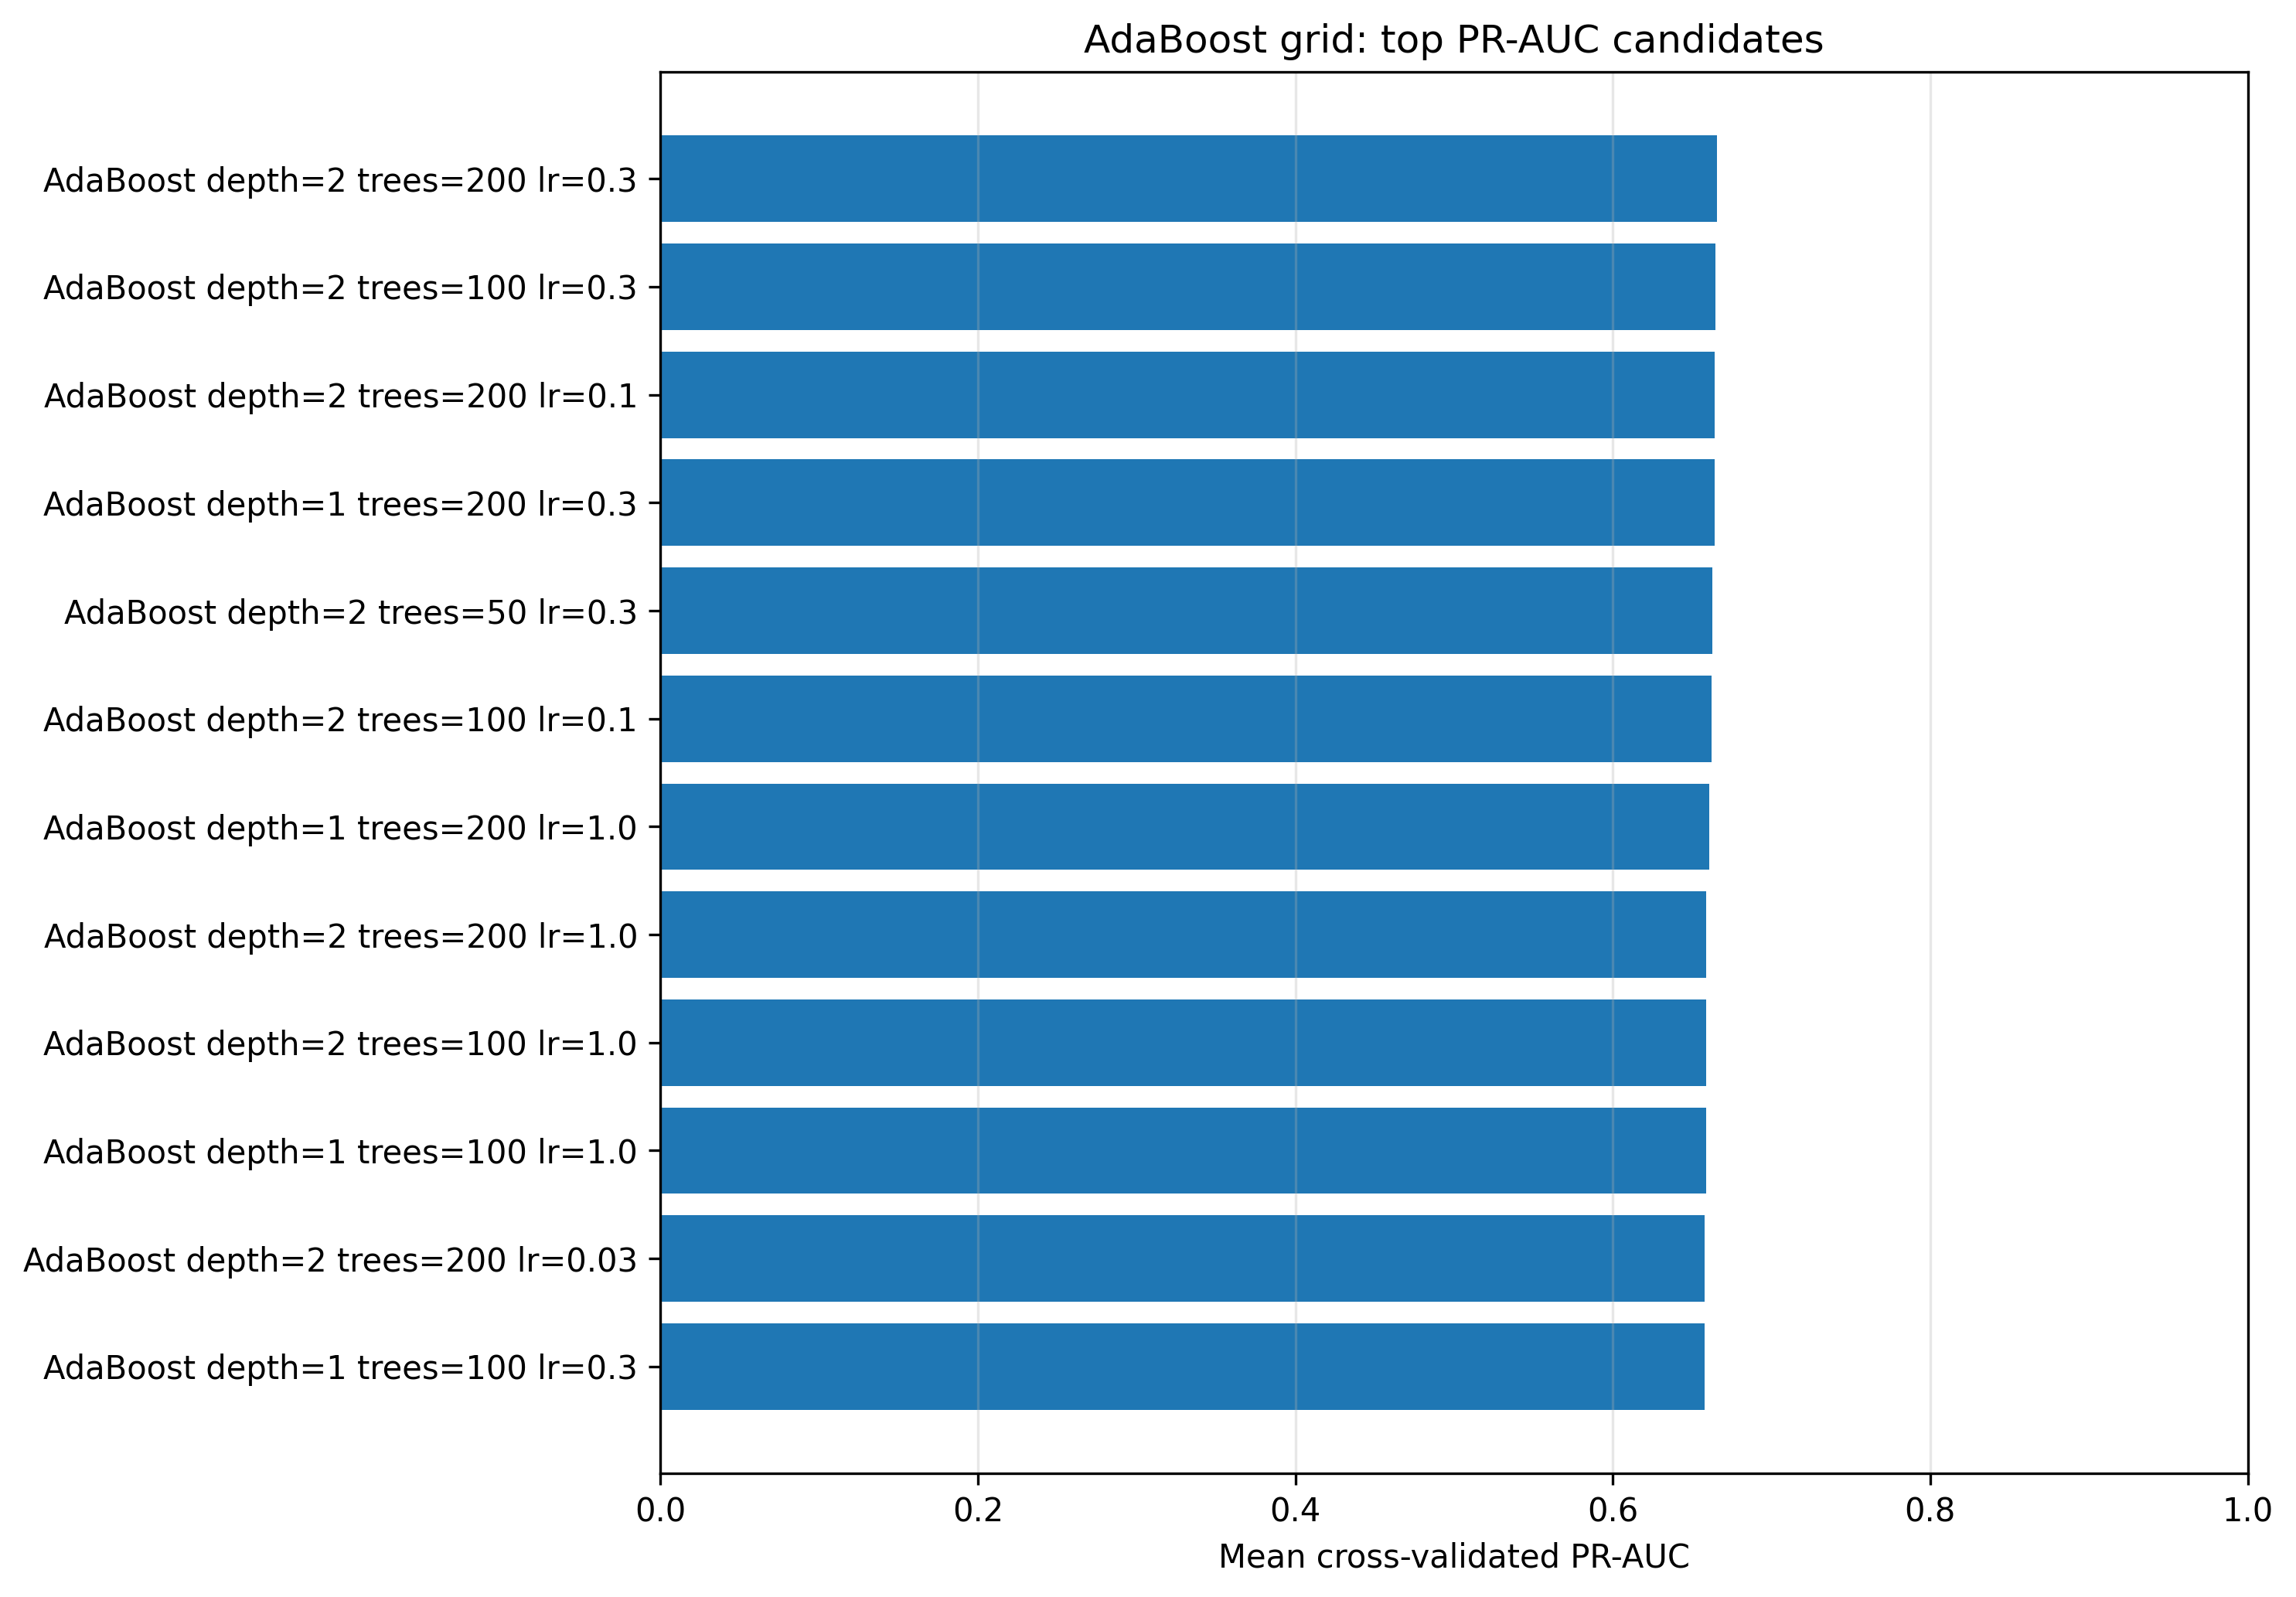
\includegraphics[width=0.88\textwidth]{../figures/adaboost_pr_auc_grid.png}
\caption{AdaBoost grid: top cross-validated PR-AUC candidates}
\label{fig:adaboost-pr-auc-grid}
\end{figure}

\begin{figure}[H]
\centering
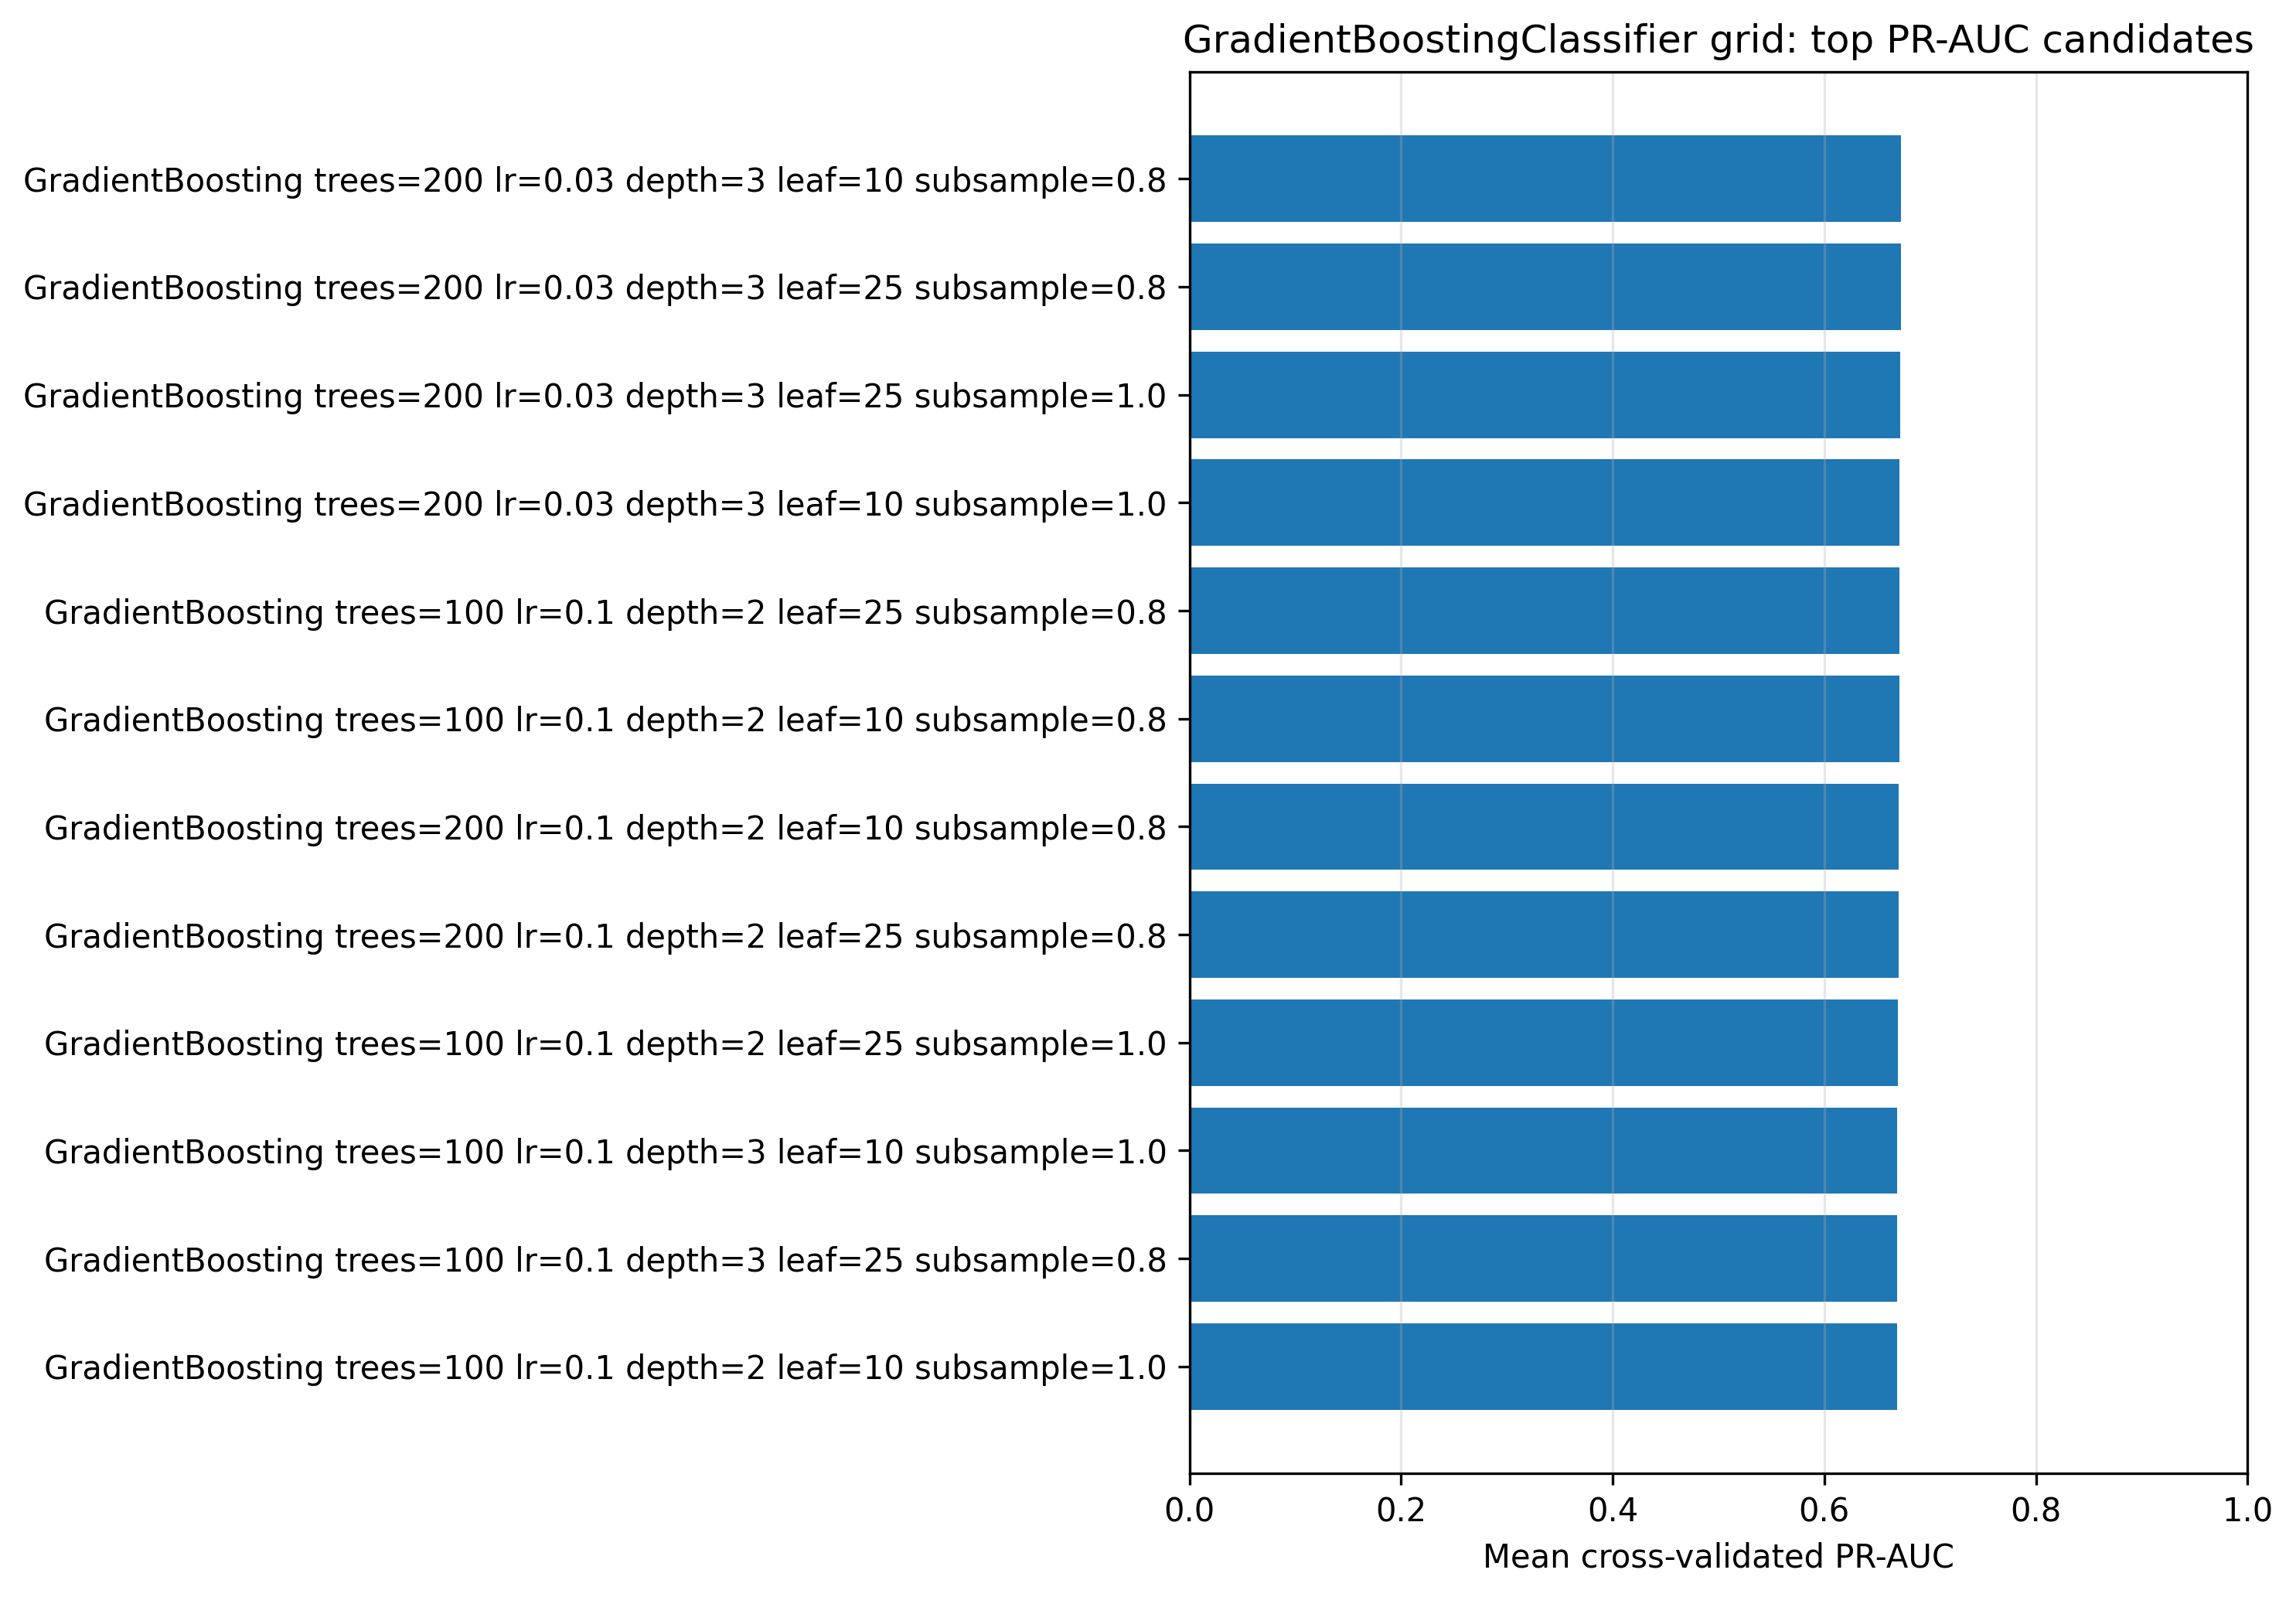
\includegraphics[width=0.88\textwidth]{../figures/gradient_boosting_pr_auc_grid.png}
\caption{GradientBoostingClassifier grid: top cross-validated PR-AUC candidates}
\label{fig:gradient-boosting-pr-auc-grid}
\end{figure}

\begin{figure}[H]
\centering
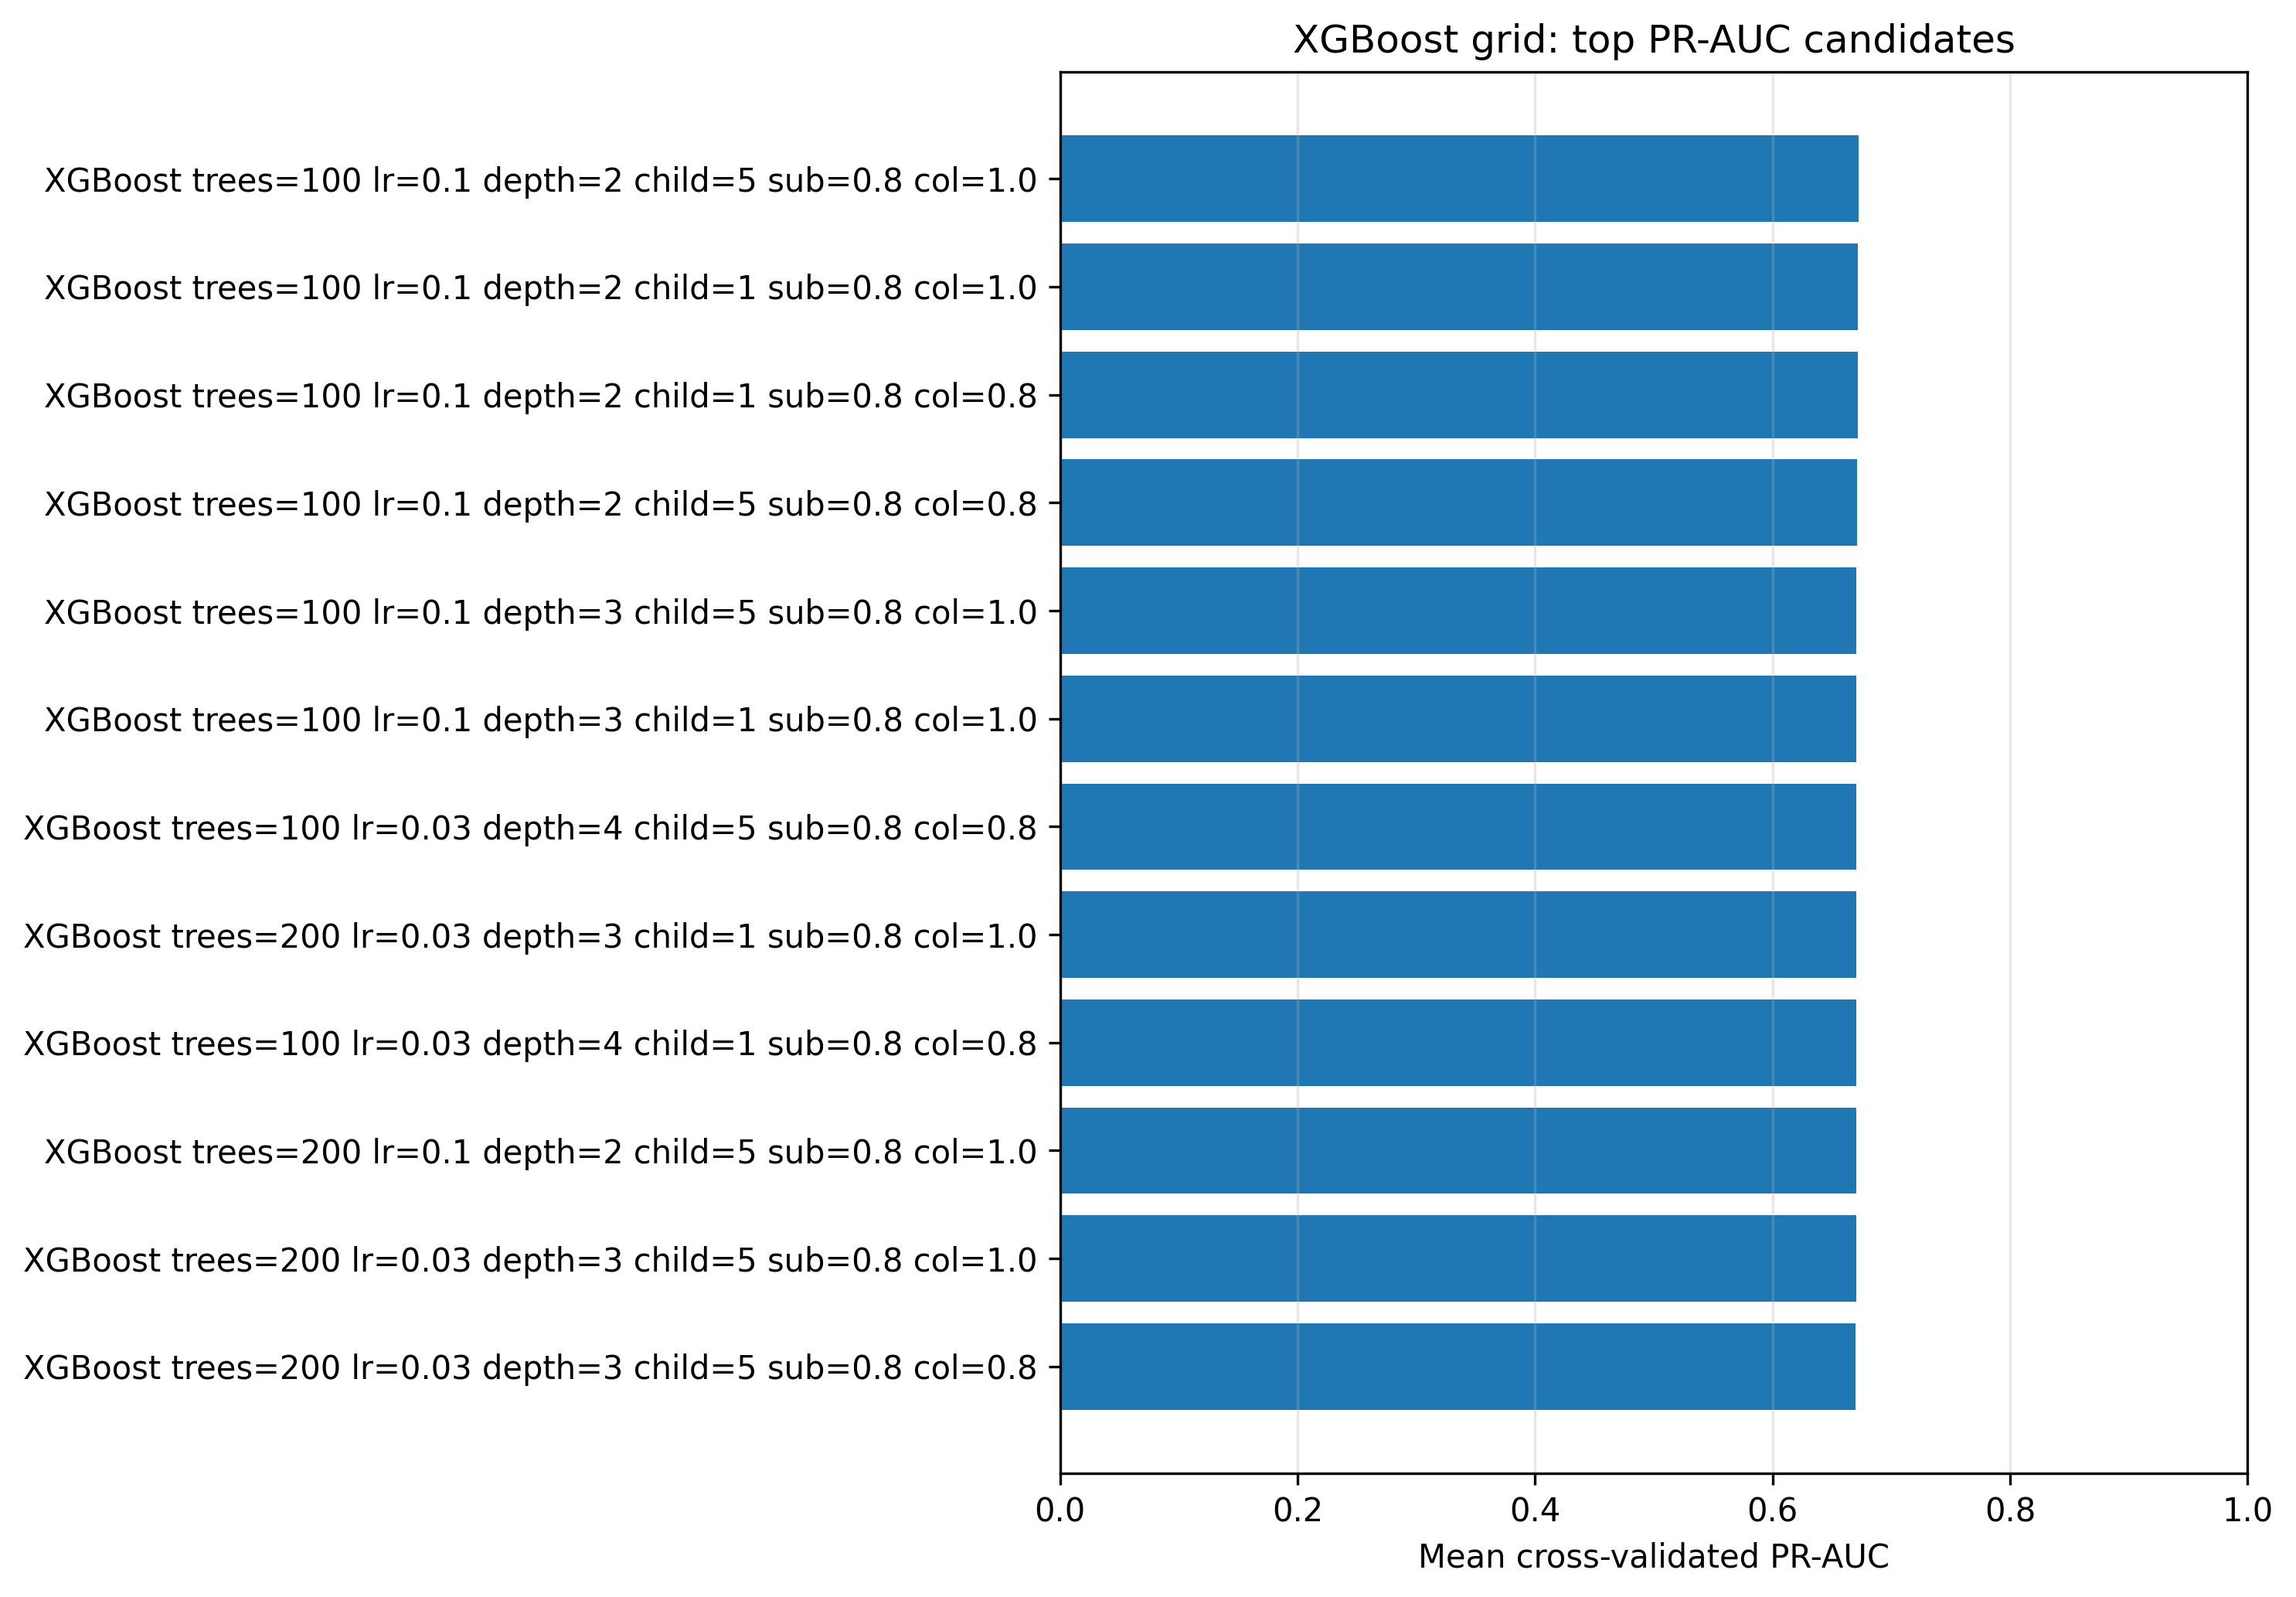
\includegraphics[width=0.88\textwidth]{../figures/xgboost_pr_auc_grid.png}
\caption{XGBoost grid: top cross-validated PR-AUC candidates}
\label{fig:xgboost-pr-auc-grid}
\end{figure}

\begin{figure}[H]
\centering
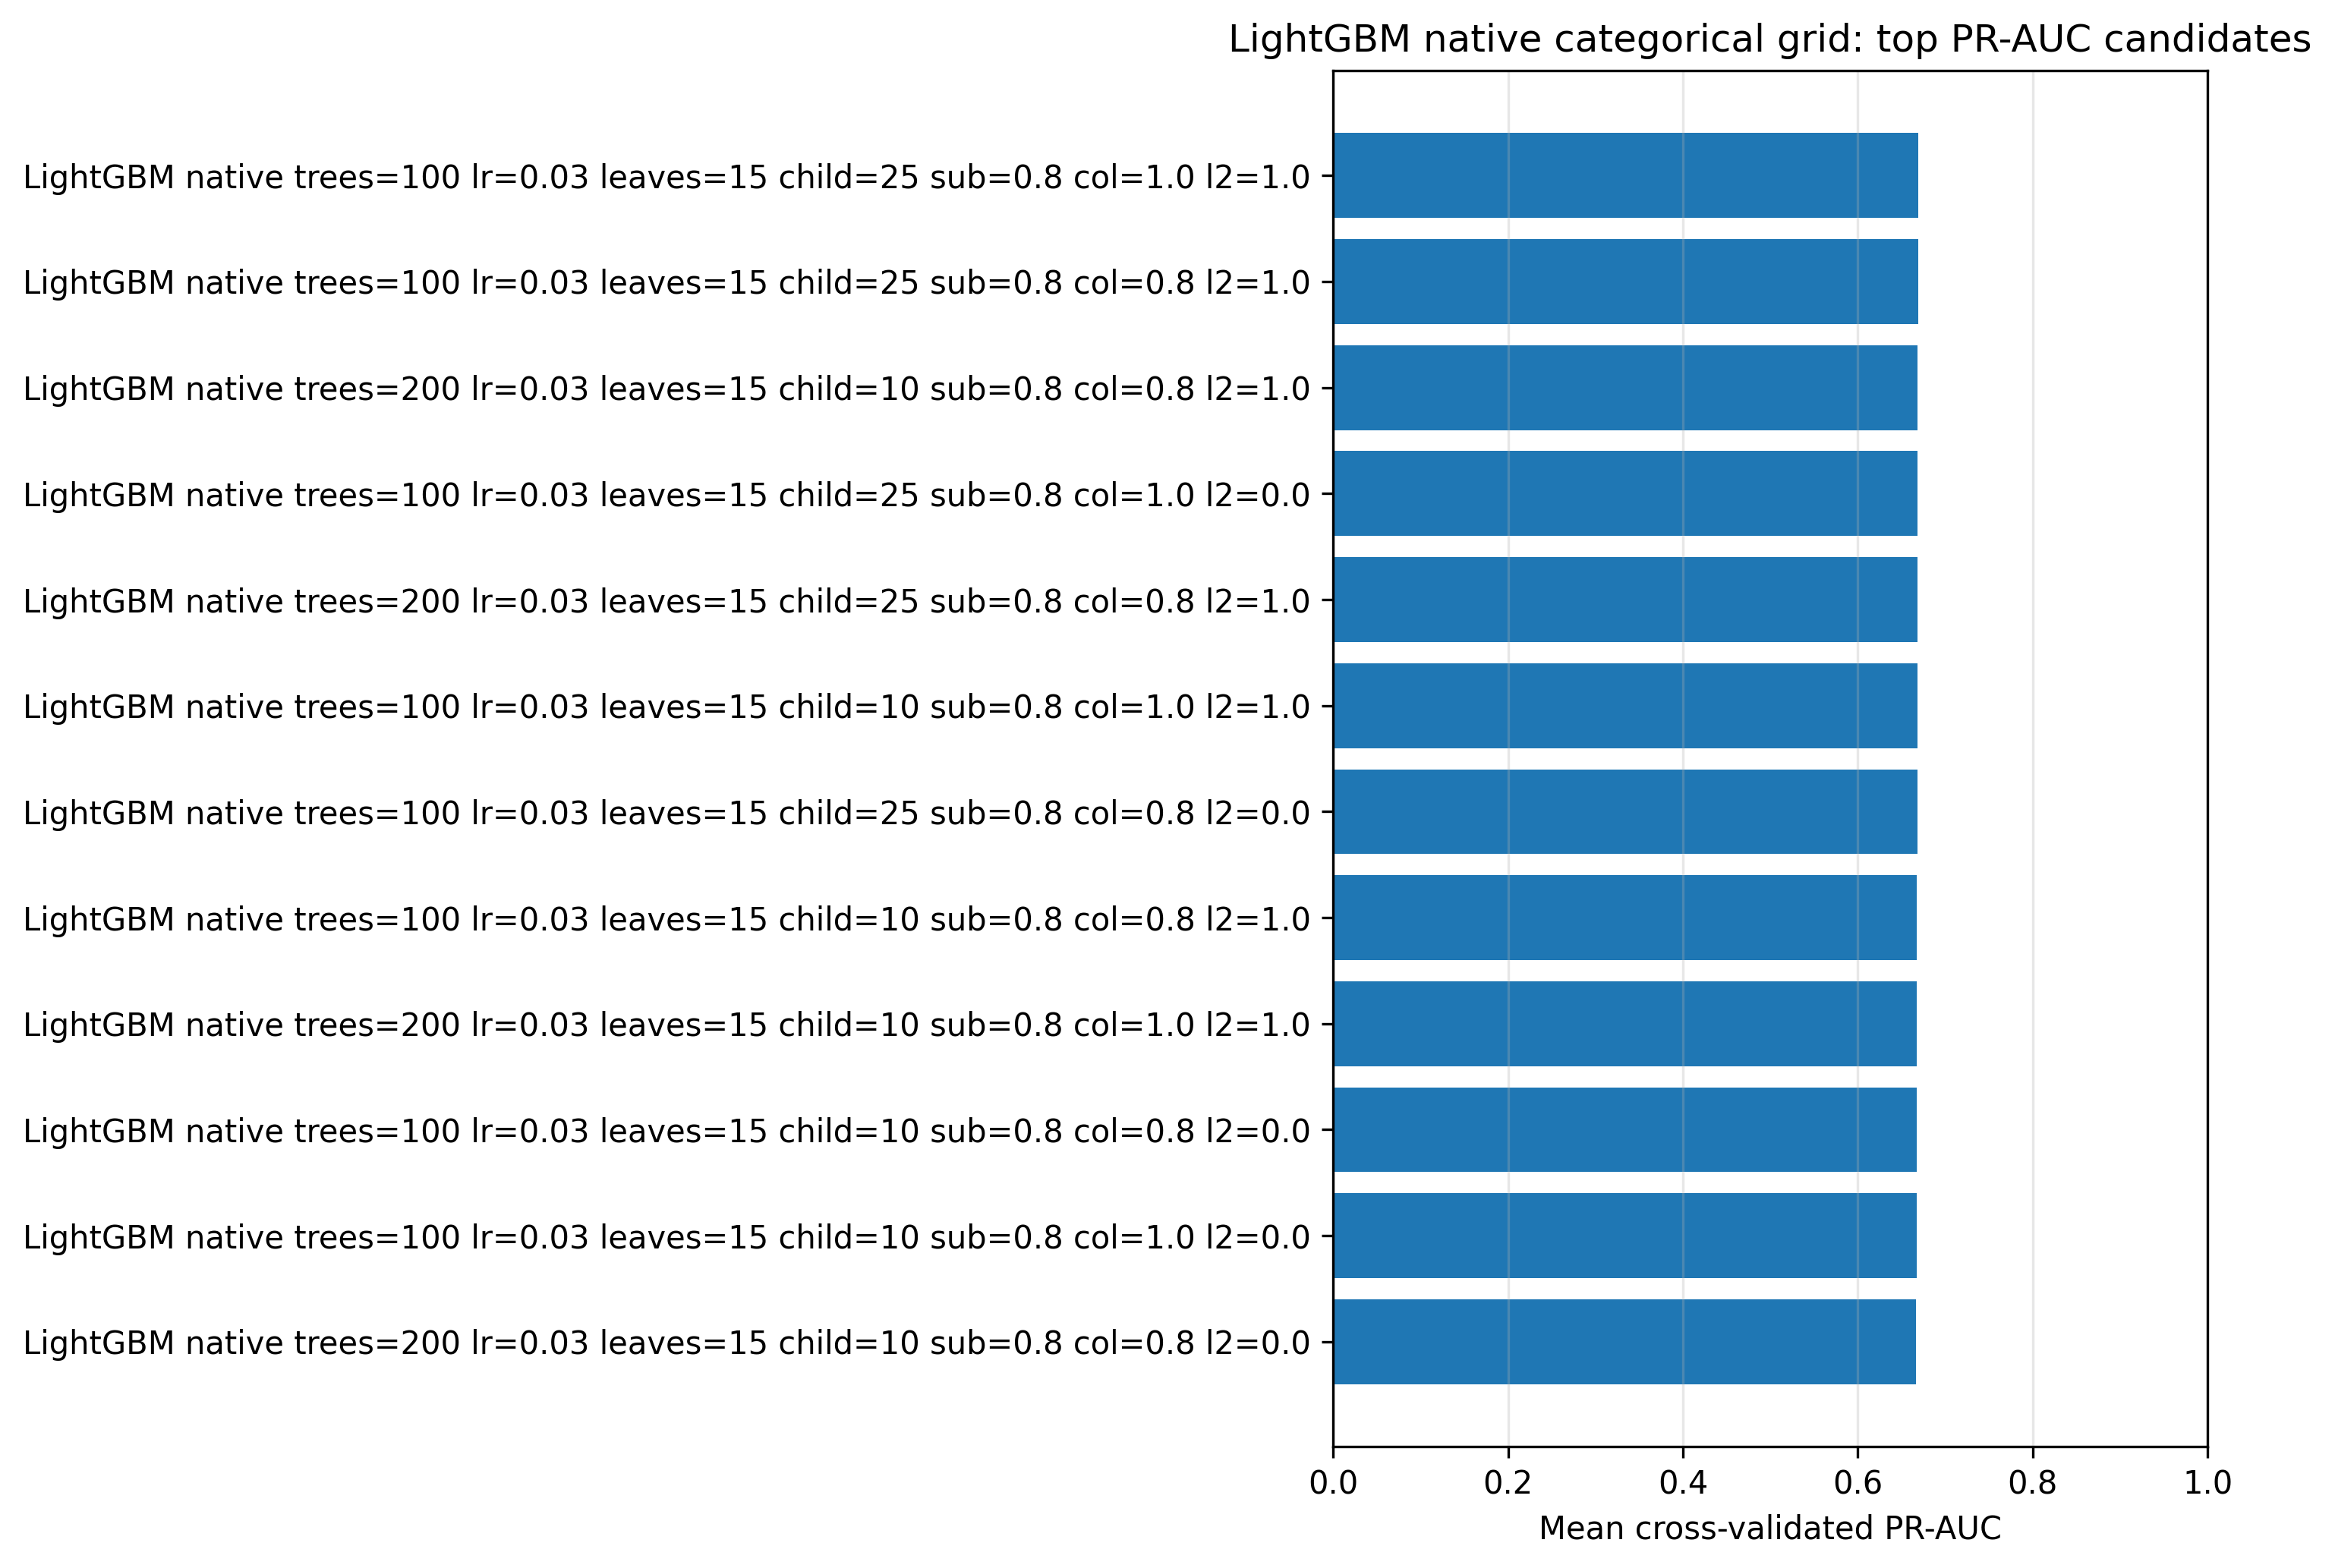
\includegraphics[width=0.88\textwidth]{../figures/lightgbm_pr_auc_grid.png}
\caption{LightGBM native categorical grid: top cross-validated PR-AUC candidates}
\label{fig:lightgbm-pr-auc-grid}
\end{figure}

\begin{figure}[H]
\centering
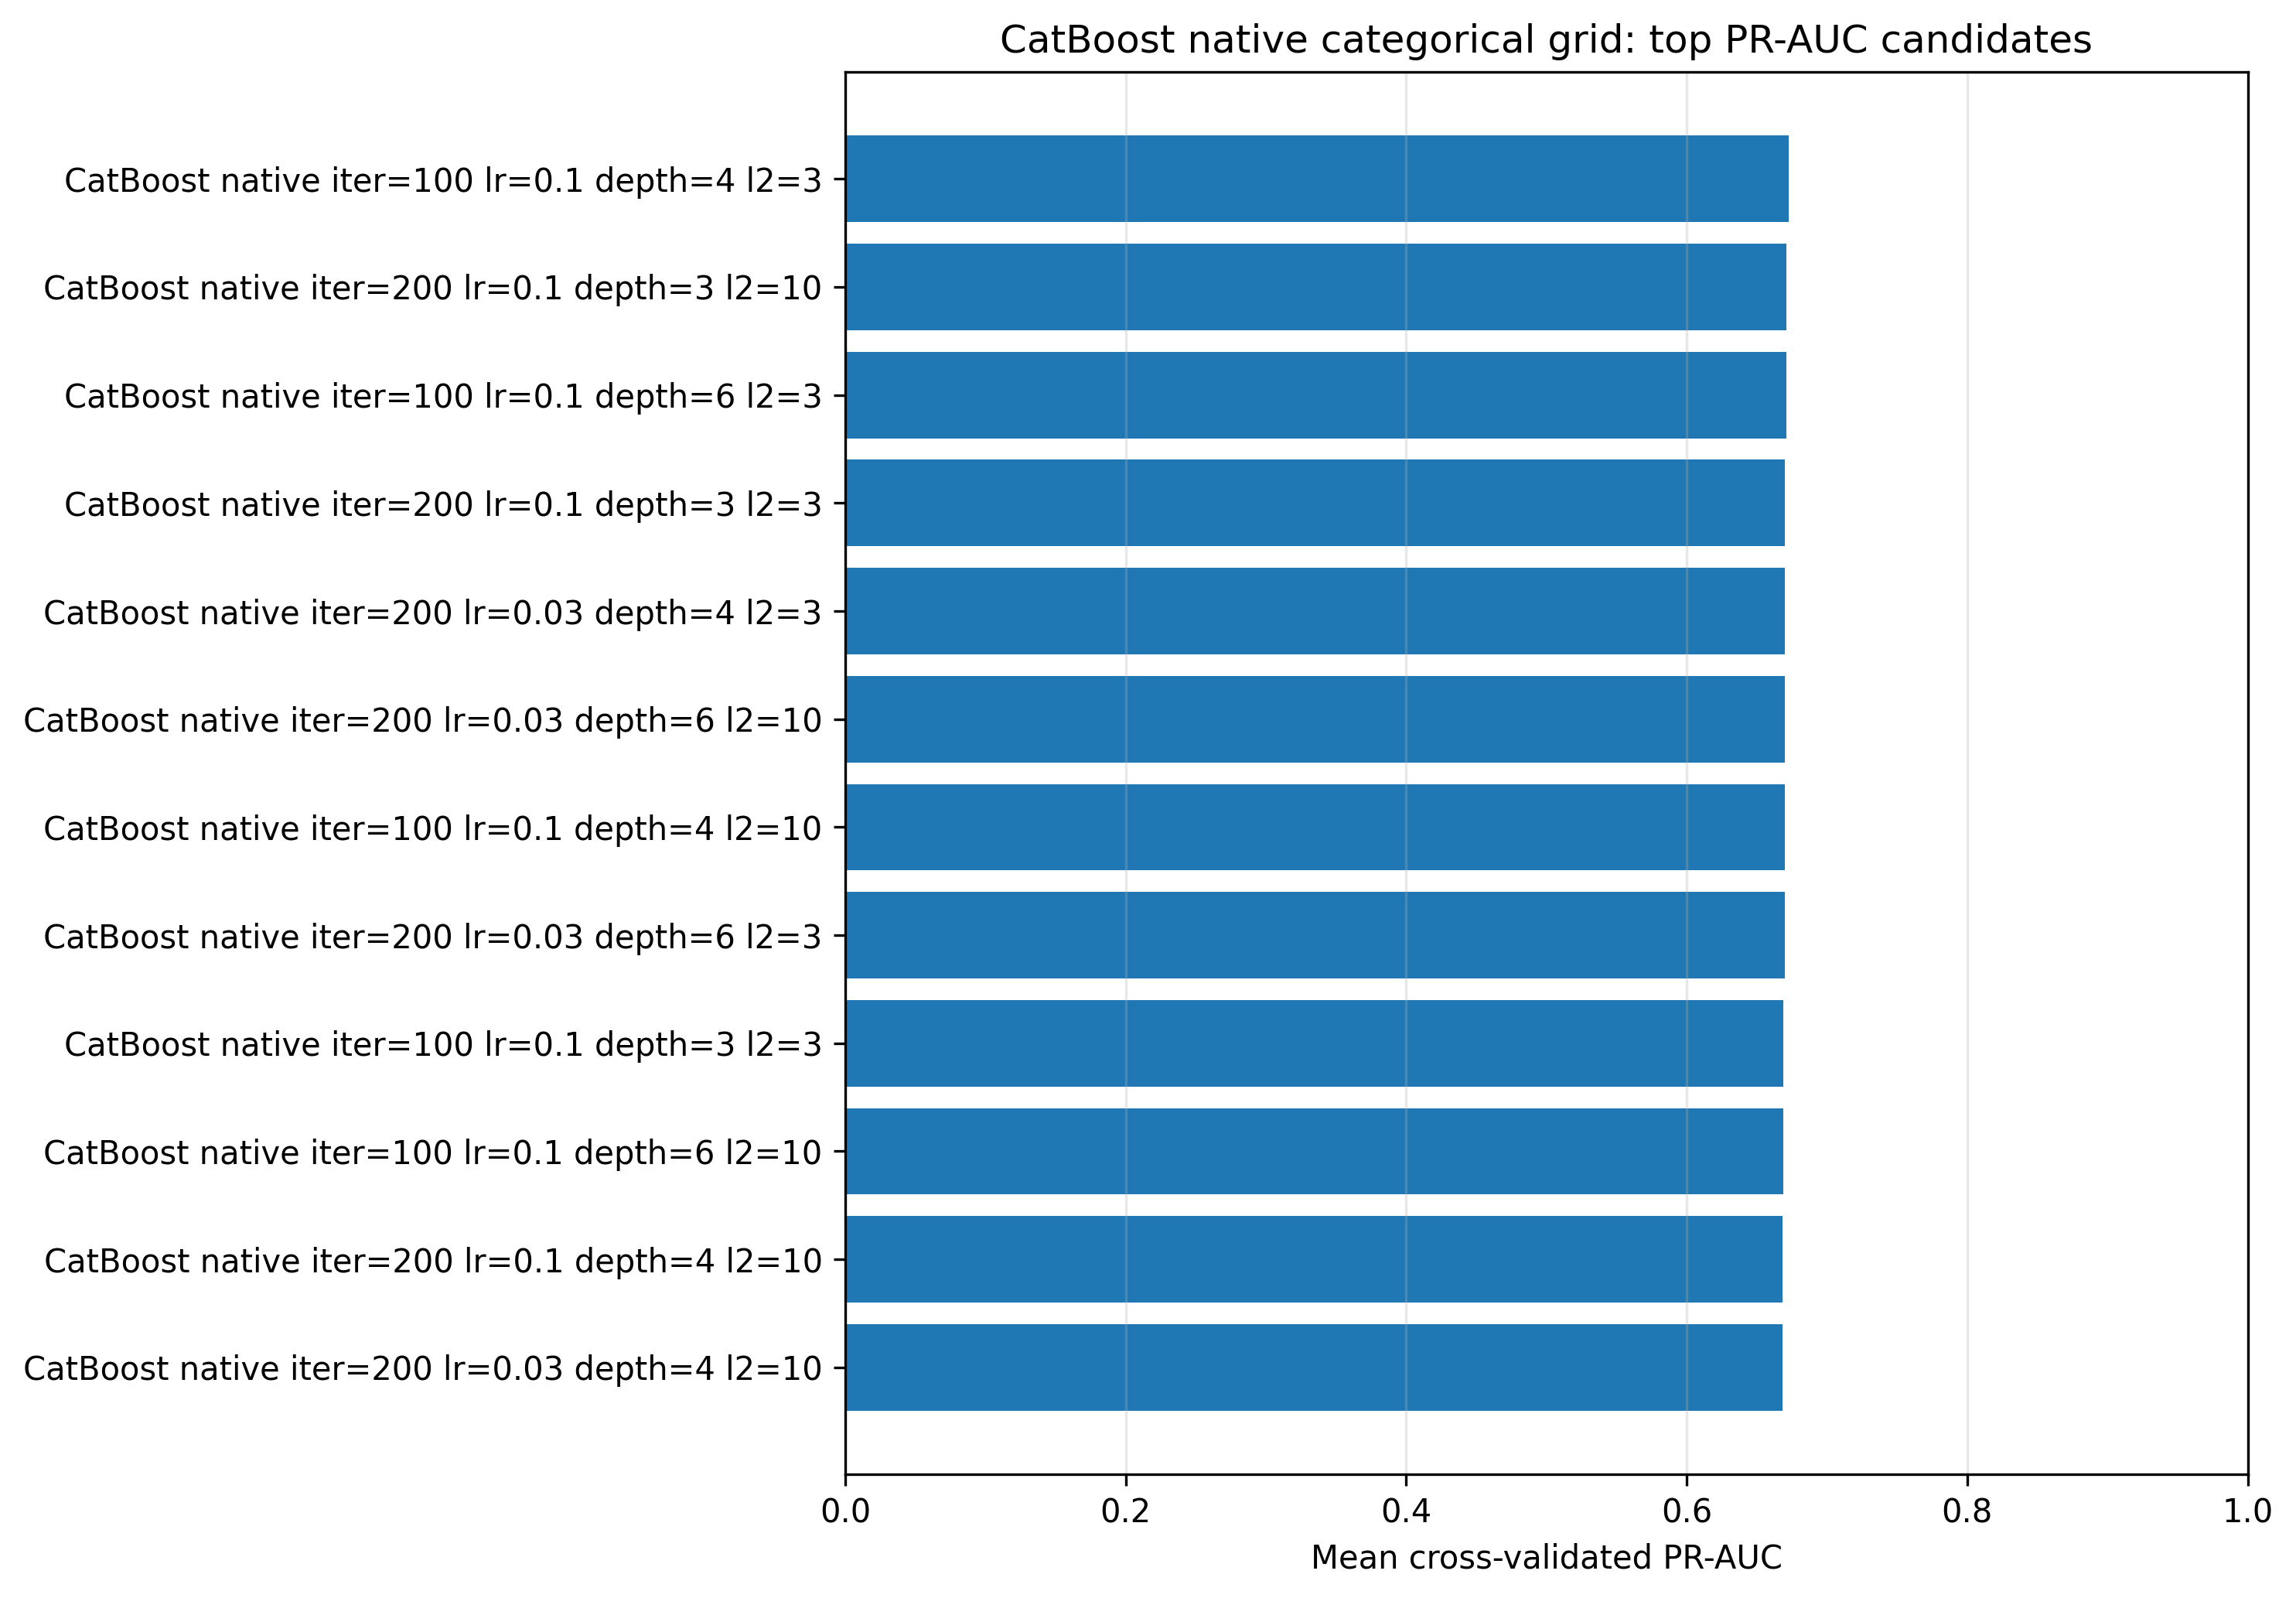
\includegraphics[width=0.88\textwidth]{../figures/catboost_pr_auc_grid.png}
\caption{CatBoost native categorical grid: top cross-validated PR-AUC candidates}
\label{fig:catboost-pr-auc-grid}
\end{figure}

\subsection{Selected candidate comparison}

After selecting one representative candidate from each boosting family, the notebook computes pooled out-of-fold predictions for each candidate and for the previous reference models. Table~\ref{tab:boosting-model-comparison} reports these pooled out-of-fold metrics.

\begin{table}[H]
\centering
\small
\resizebox{\textwidth}{!}{
\begin{tabular}{lrrrrrrrr}
\toprule
Model & Accuracy & Bal. Acc. & Precision & Recall & Specificity & \(F_1\) & ROC-AUC & PR-AUC \\
\midrule
Best XGBoost & 0.808 & 0.722 & 0.671 & 0.539 & 0.905 & 0.598 & 0.850 & 0.670 \\
Best GradientBoostingClassifier & 0.808 & 0.719 & 0.677 & 0.530 & 0.908 & 0.595 & 0.850 & 0.669 \\
Best CatBoost native categorical & 0.807 & 0.717 & 0.676 & 0.525 & 0.909 & 0.591 & 0.850 & 0.669 \\
Best LightGBM native categorical & 0.804 & 0.711 & 0.672 & 0.512 & 0.910 & 0.581 & 0.849 & 0.666 \\
Best AdaBoost & 0.805 & 0.718 & 0.666 & 0.533 & 0.903 & 0.592 & 0.848 & 0.664 \\
Selected bagged trees & 0.800 & 0.705 & 0.662 & 0.504 & 0.907 & 0.572 & 0.846 & 0.662 \\
Selected random forest & 0.804 & 0.706 & 0.678 & 0.498 & 0.914 & 0.574 & 0.847 & 0.660 \\
Best HistGradientBoostingClassifier & 0.807 & 0.719 & 0.671 & 0.532 & 0.906 & 0.594 & 0.848 & 0.660 \\
Selected L2 logistic regression & 0.802 & 0.719 & 0.652 & 0.544 & 0.895 & 0.593 & 0.846 & 0.658 \\
Selected single decision tree & 0.789 & 0.701 & 0.624 & 0.514 & 0.888 & 0.564 & 0.824 & 0.628 \\
\bottomrule
\end{tabular}
}
\caption{Pooled out-of-fold comparison of selected boosting candidates and reference models}
\label{tab:boosting-model-comparison}
\end{table}

Figure~\ref{fig:boosting-model-comparison-pr-auc} shows the same comparison by PR-AUC. XGBoost ranks first in this pooled out-of-fold comparison, with PR-AUC approximately \(0.670\). \texttt{GradientBoostingClassifier} and CatBoost follow extremely closely, both at approximately \(0.669\). LightGBM and AdaBoost are slightly lower, while the selected bagged trees, selected random forest, and selected L2 logistic regression are close to one another around \(0.658\) to \(0.662\). The single decision tree remains clearly weaker by PR-AUC.

\begin{figure}[H]
\centering
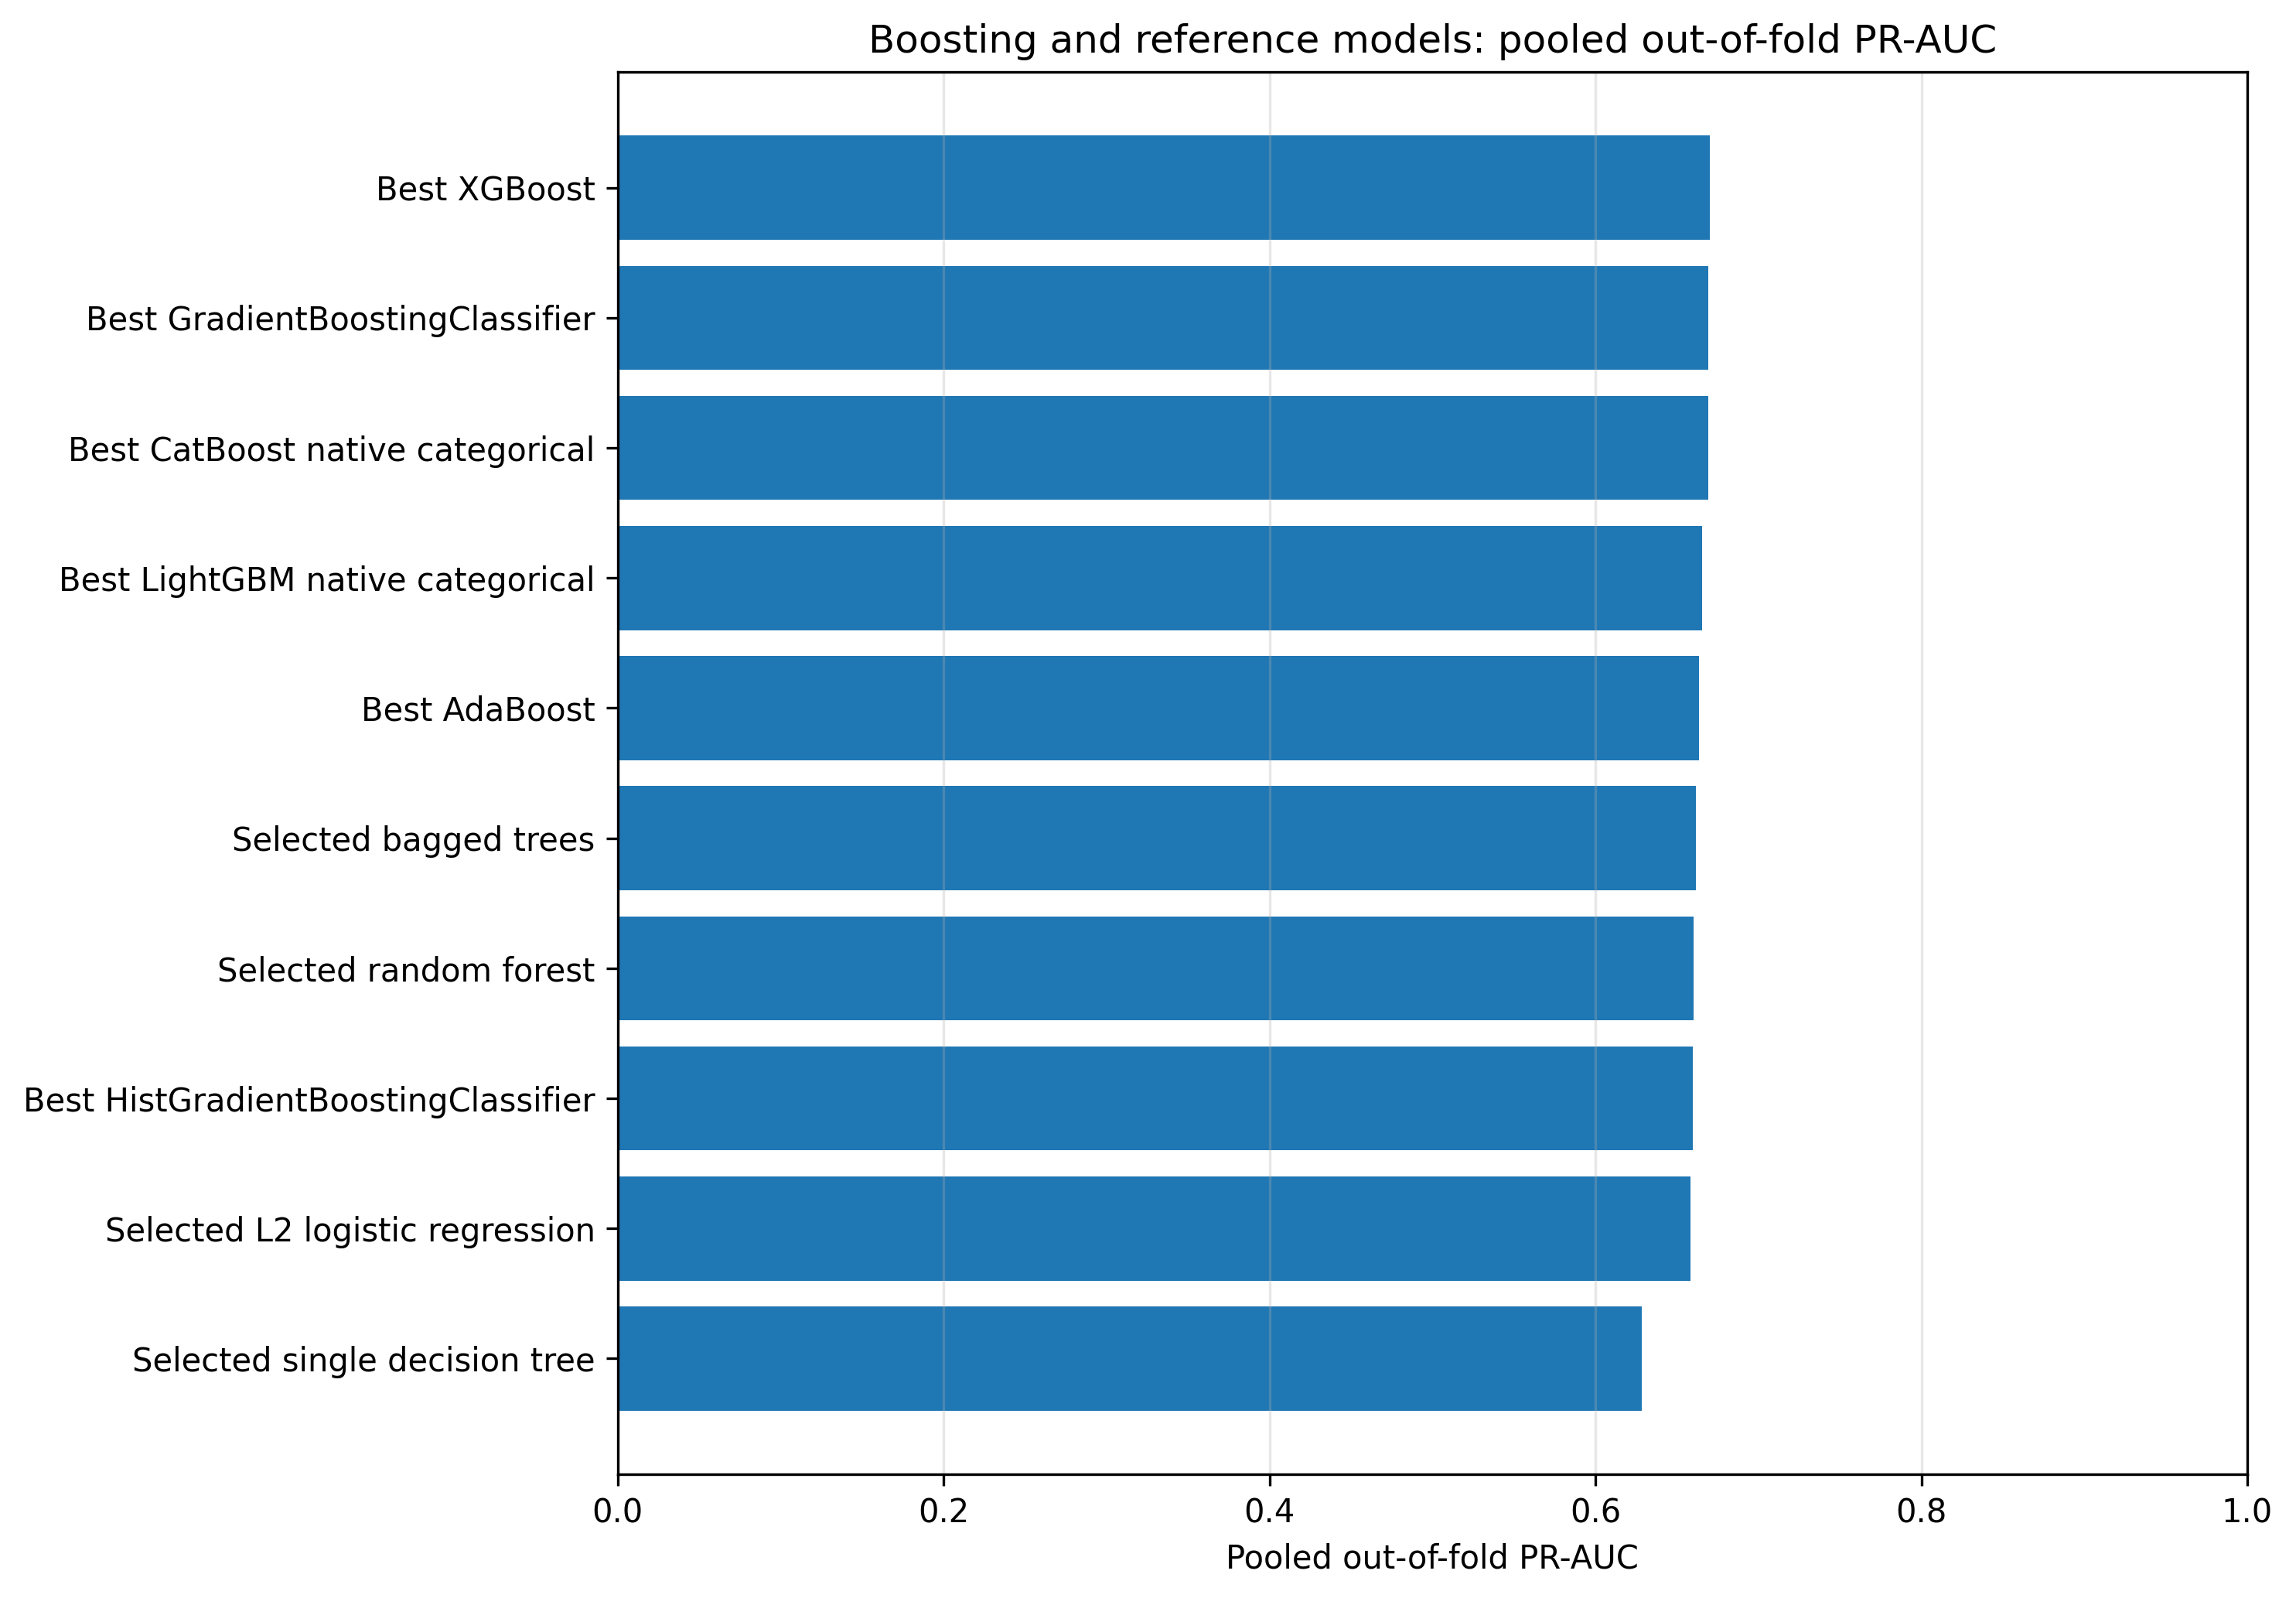
\includegraphics[width=0.88\textwidth]{../figures/boosting_model_comparison_pr_auc.png}
\caption{Boosting and reference models: pooled out-of-fold PR-AUC}
\label{fig:boosting-model-comparison-pr-auc}
\end{figure}

The main conclusion is that boosting forms the strongest development-stage group in this section. The improvement over the single tree is clear. The improvement over bagging, random forests, and logistic regression is more modest. The difference between XGBoost and the next two boosting candidates is too small to claim a meaningful ordering. This section therefore identifies XGBoost as the representative boosting diagnostic model by the chosen pooled out-of-fold PR-AUC rule, but it does not claim that XGBoost has been proven superior to the other leading boosted tree implementations.

\subsection{Confusion-matrix behaviour}

Table~\ref{tab:boosting-confusion-matrices} reports positive-first confusion-matrix counts at the default threshold. The selected XGBoost model detects \(806\) of the \(1495\) churners and produces \(395\) false positives. This corresponds to recall approximately \(0.539\), precision approximately \(0.671\), and a predicted positive rate of approximately \(0.213\), below the observed churn rate of approximately \(0.265\).

\begin{table}[H]
\centering
\small
\resizebox{\textwidth}{!}{
\begin{tabular}{lrrrrr}
\toprule
Model & TP & FN & FP & TN & Pred. positive rate \\
\midrule
Best XGBoost & 806 & 689 & 395 & 3744 & 0.213 \\
Best GradientBoostingClassifier & 793 & 702 & 379 & 3760 & 0.208 \\
Best CatBoost native categorical & 785 & 710 & 377 & 3762 & 0.206 \\
Best LightGBM native categorical & 765 & 730 & 373 & 3766 & 0.202 \\
Best AdaBoost & 797 & 698 & 400 & 3739 & 0.212 \\
Selected bagged trees & 753 & 742 & 385 & 3754 & 0.202 \\
Selected random forest & 744 & 751 & 354 & 3785 & 0.195 \\
Best HistGradientBoostingClassifier & 796 & 699 & 391 & 3748 & 0.211 \\
Selected L2 logistic regression & 813 & 682 & 434 & 3705 & 0.221 \\
Selected single decision tree & 769 & 726 & 463 & 3676 & 0.219 \\
\bottomrule
\end{tabular}
}
\caption{Positive-first pooled out-of-fold confusion-matrix counts for selected boosting candidates and reference models}
\label{tab:boosting-confusion-matrices}
\end{table}

The default-threshold behaviour shows that many of the strongest candidates are relatively conservative. They flag fewer customers than the observed churn proportion. Logistic regression detects slightly more churners at the default threshold, but it also produces more false positives and has lower PR-AUC than the top boosting models. This reinforces the distinction between ranking performance and operating-threshold performance. A model can rank customers well while still requiring a threshold adjustment if the business objective prioritizes recall.

\subsection{Threshold behaviour for the selected XGBoost model}

The selected XGBoost model is used for threshold diagnostics because it has the highest pooled out-of-fold PR-AUC in Table~\ref{tab:boosting-model-comparison}. Table~\ref{tab:boosting-threshold-results} reports selected thresholds. Lower thresholds recover more churners but also flag many more non-churners. Higher thresholds increase precision and specificity but miss more churners.

\begin{table}[H]
\centering
\small
\begin{tabular}{rrrrrr}
\toprule
Threshold & Precision & Recall & Specificity & \(F_1\) & Pred. positive rate \\
\midrule
0.100 & 0.406 & 0.940 & 0.504 & 0.567 & 0.614 \\
0.200 & 0.485 & 0.865 & 0.669 & 0.622 & 0.473 \\
0.250 & 0.512 & 0.824 & 0.716 & 0.631 & 0.427 \\
0.300 & 0.541 & 0.771 & 0.763 & 0.636 & 0.378 \\
0.350 & 0.572 & 0.716 & 0.806 & 0.636 & 0.332 \\
0.400 & 0.611 & 0.655 & 0.849 & 0.632 & 0.285 \\
0.500 & 0.671 & 0.539 & 0.905 & 0.598 & 0.213 \\
0.600 & 0.718 & 0.379 & 0.946 & 0.496 & 0.140 \\
\bottomrule
\end{tabular}
\caption{Threshold behaviour for the selected XGBoost model using pooled out-of-fold scores}
\label{tab:boosting-threshold-results}
\end{table}

At the default threshold \(0.50\), precision is about \(0.671\), recall is about \(0.539\), and \(F_1\) is about \(0.598\). Lowering the threshold to \(0.30\) increases recall to about \(0.771\) and gives \(F_1\) about \(0.636\), but precision falls to about \(0.541\). A threshold near \(0.25\) gives even higher recall, about \(0.824\), but flags approximately \(42.7\%\) of customers. These patterns are expected for an imbalanced churn problem. A lower threshold can be reasonable if missed churners are expensive, but the final threshold should not be chosen in this section. It depends on intervention costs, retention value, capacity constraints, calibration, and final model comparison.

Figure~\ref{fig:boosting-threshold-tradeoff} visualizes the same tradeoff.

\begin{figure}[H]
\centering
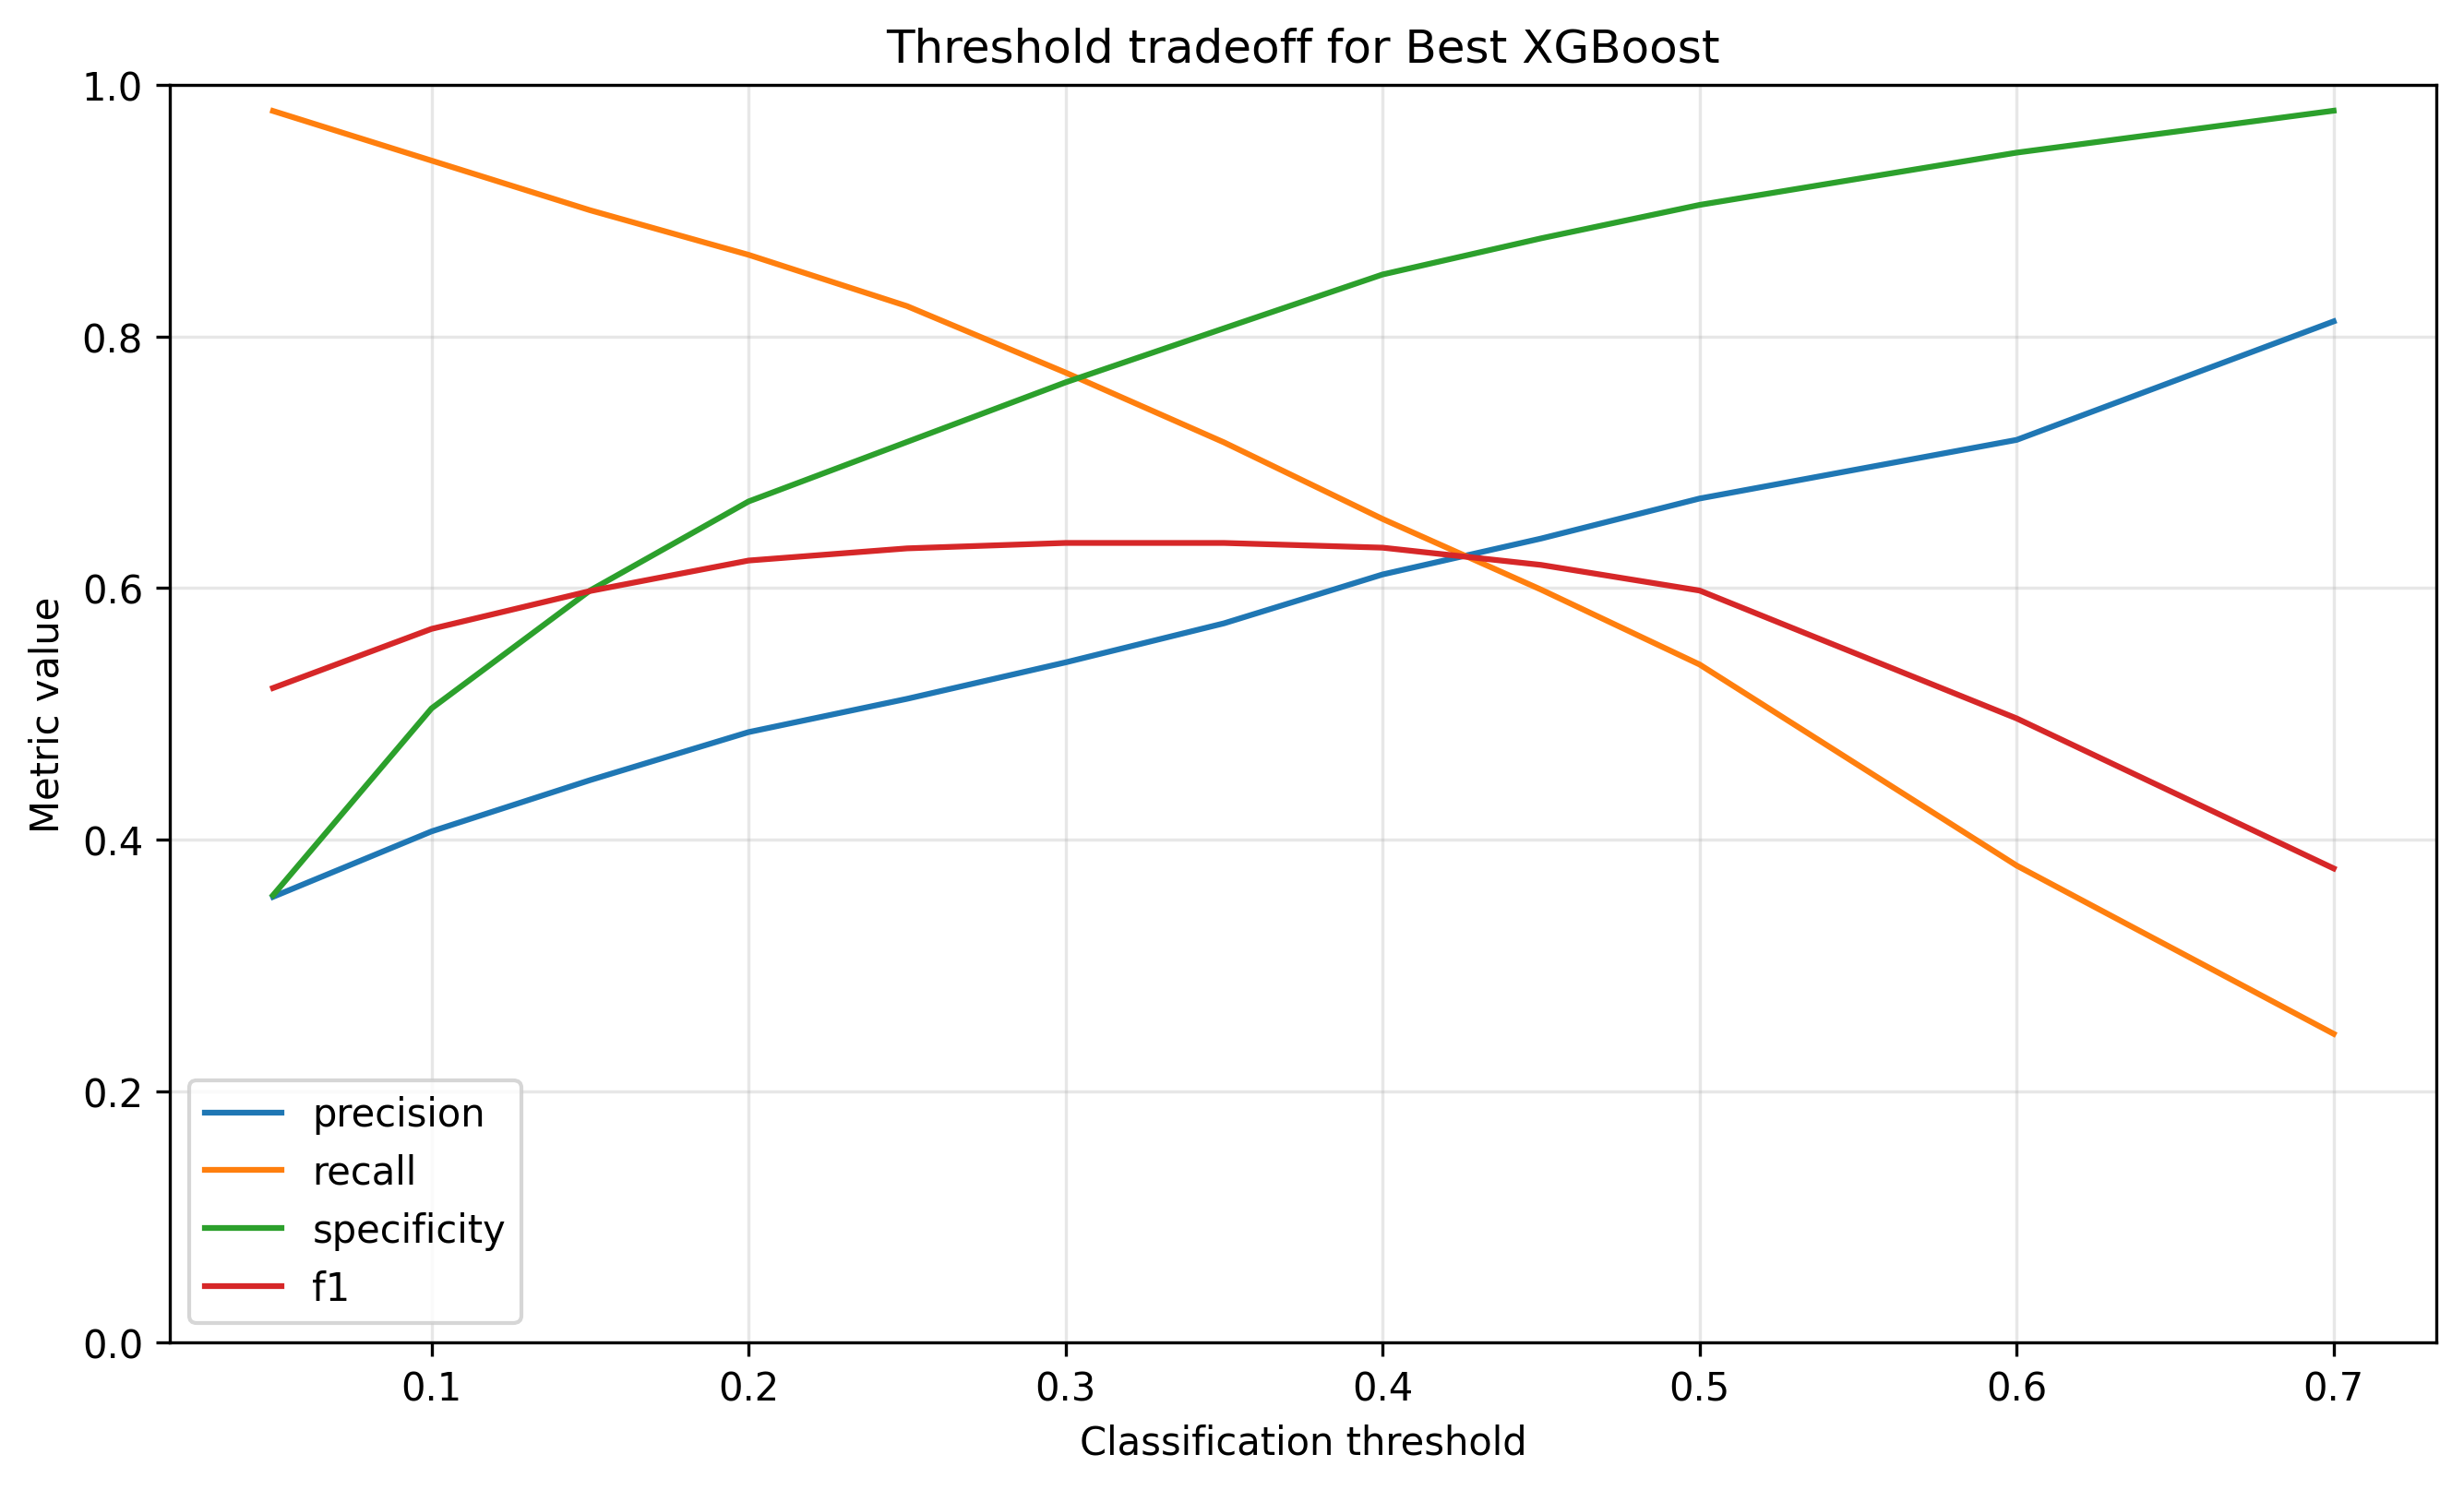
\includegraphics[width=0.88\textwidth]{../figures/boosting_threshold_tradeoff.png}
\caption{Threshold tradeoff for the selected XGBoost model}
\label{fig:boosting-threshold-tradeoff}
\end{figure}

\subsection{Ranking curves}

Figures~\ref{fig:boosting-roc-curve} and~\ref{fig:boosting-pr-curve} show the ROC and precision-recall curves for the selected XGBoost model. The ROC-AUC is approximately \(0.850\), while the PR-AUC is approximately \(0.670\). The precision-recall curve remains well above the positive-rate baseline of approximately \(0.265\) over much of the recall range, indicating that the model produces useful churn-risk rankings.

\begin{figure}[H]
\centering
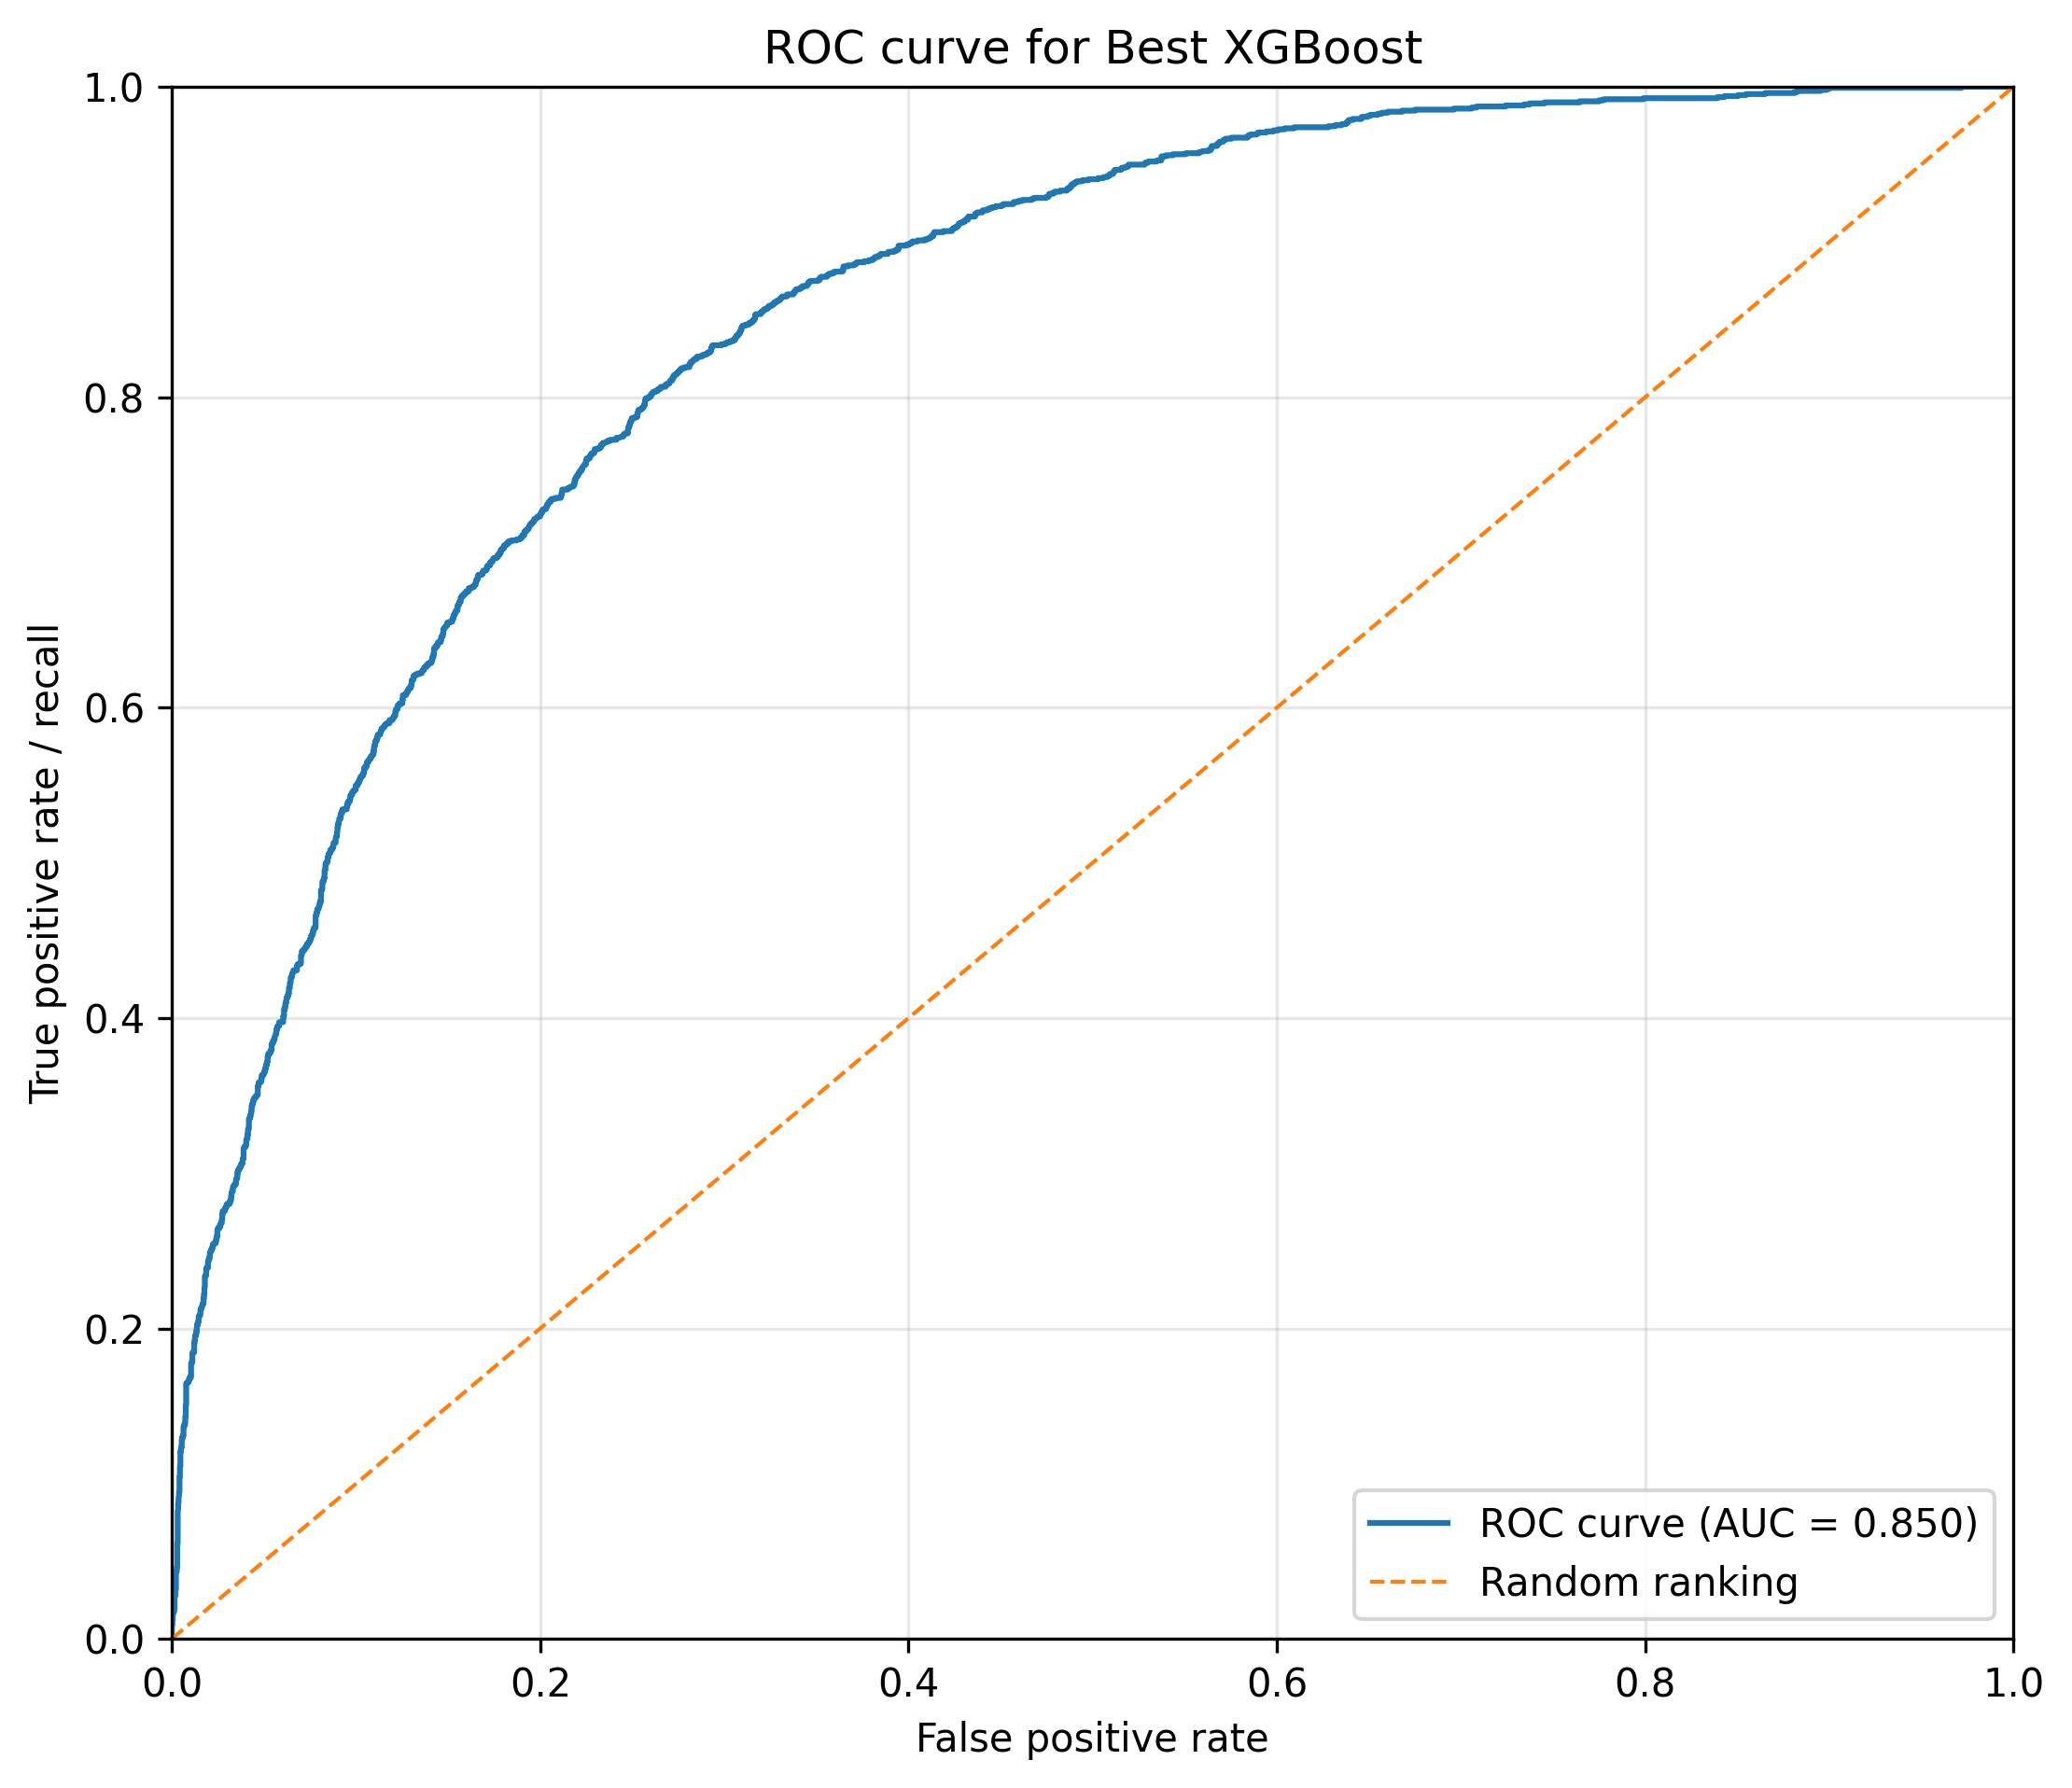
\includegraphics[width=0.82\textwidth]{../figures/boosting_roc_curve.png}
\caption{ROC curve for the selected XGBoost model}
\label{fig:boosting-roc-curve}
\end{figure}

\begin{figure}[H]
\centering
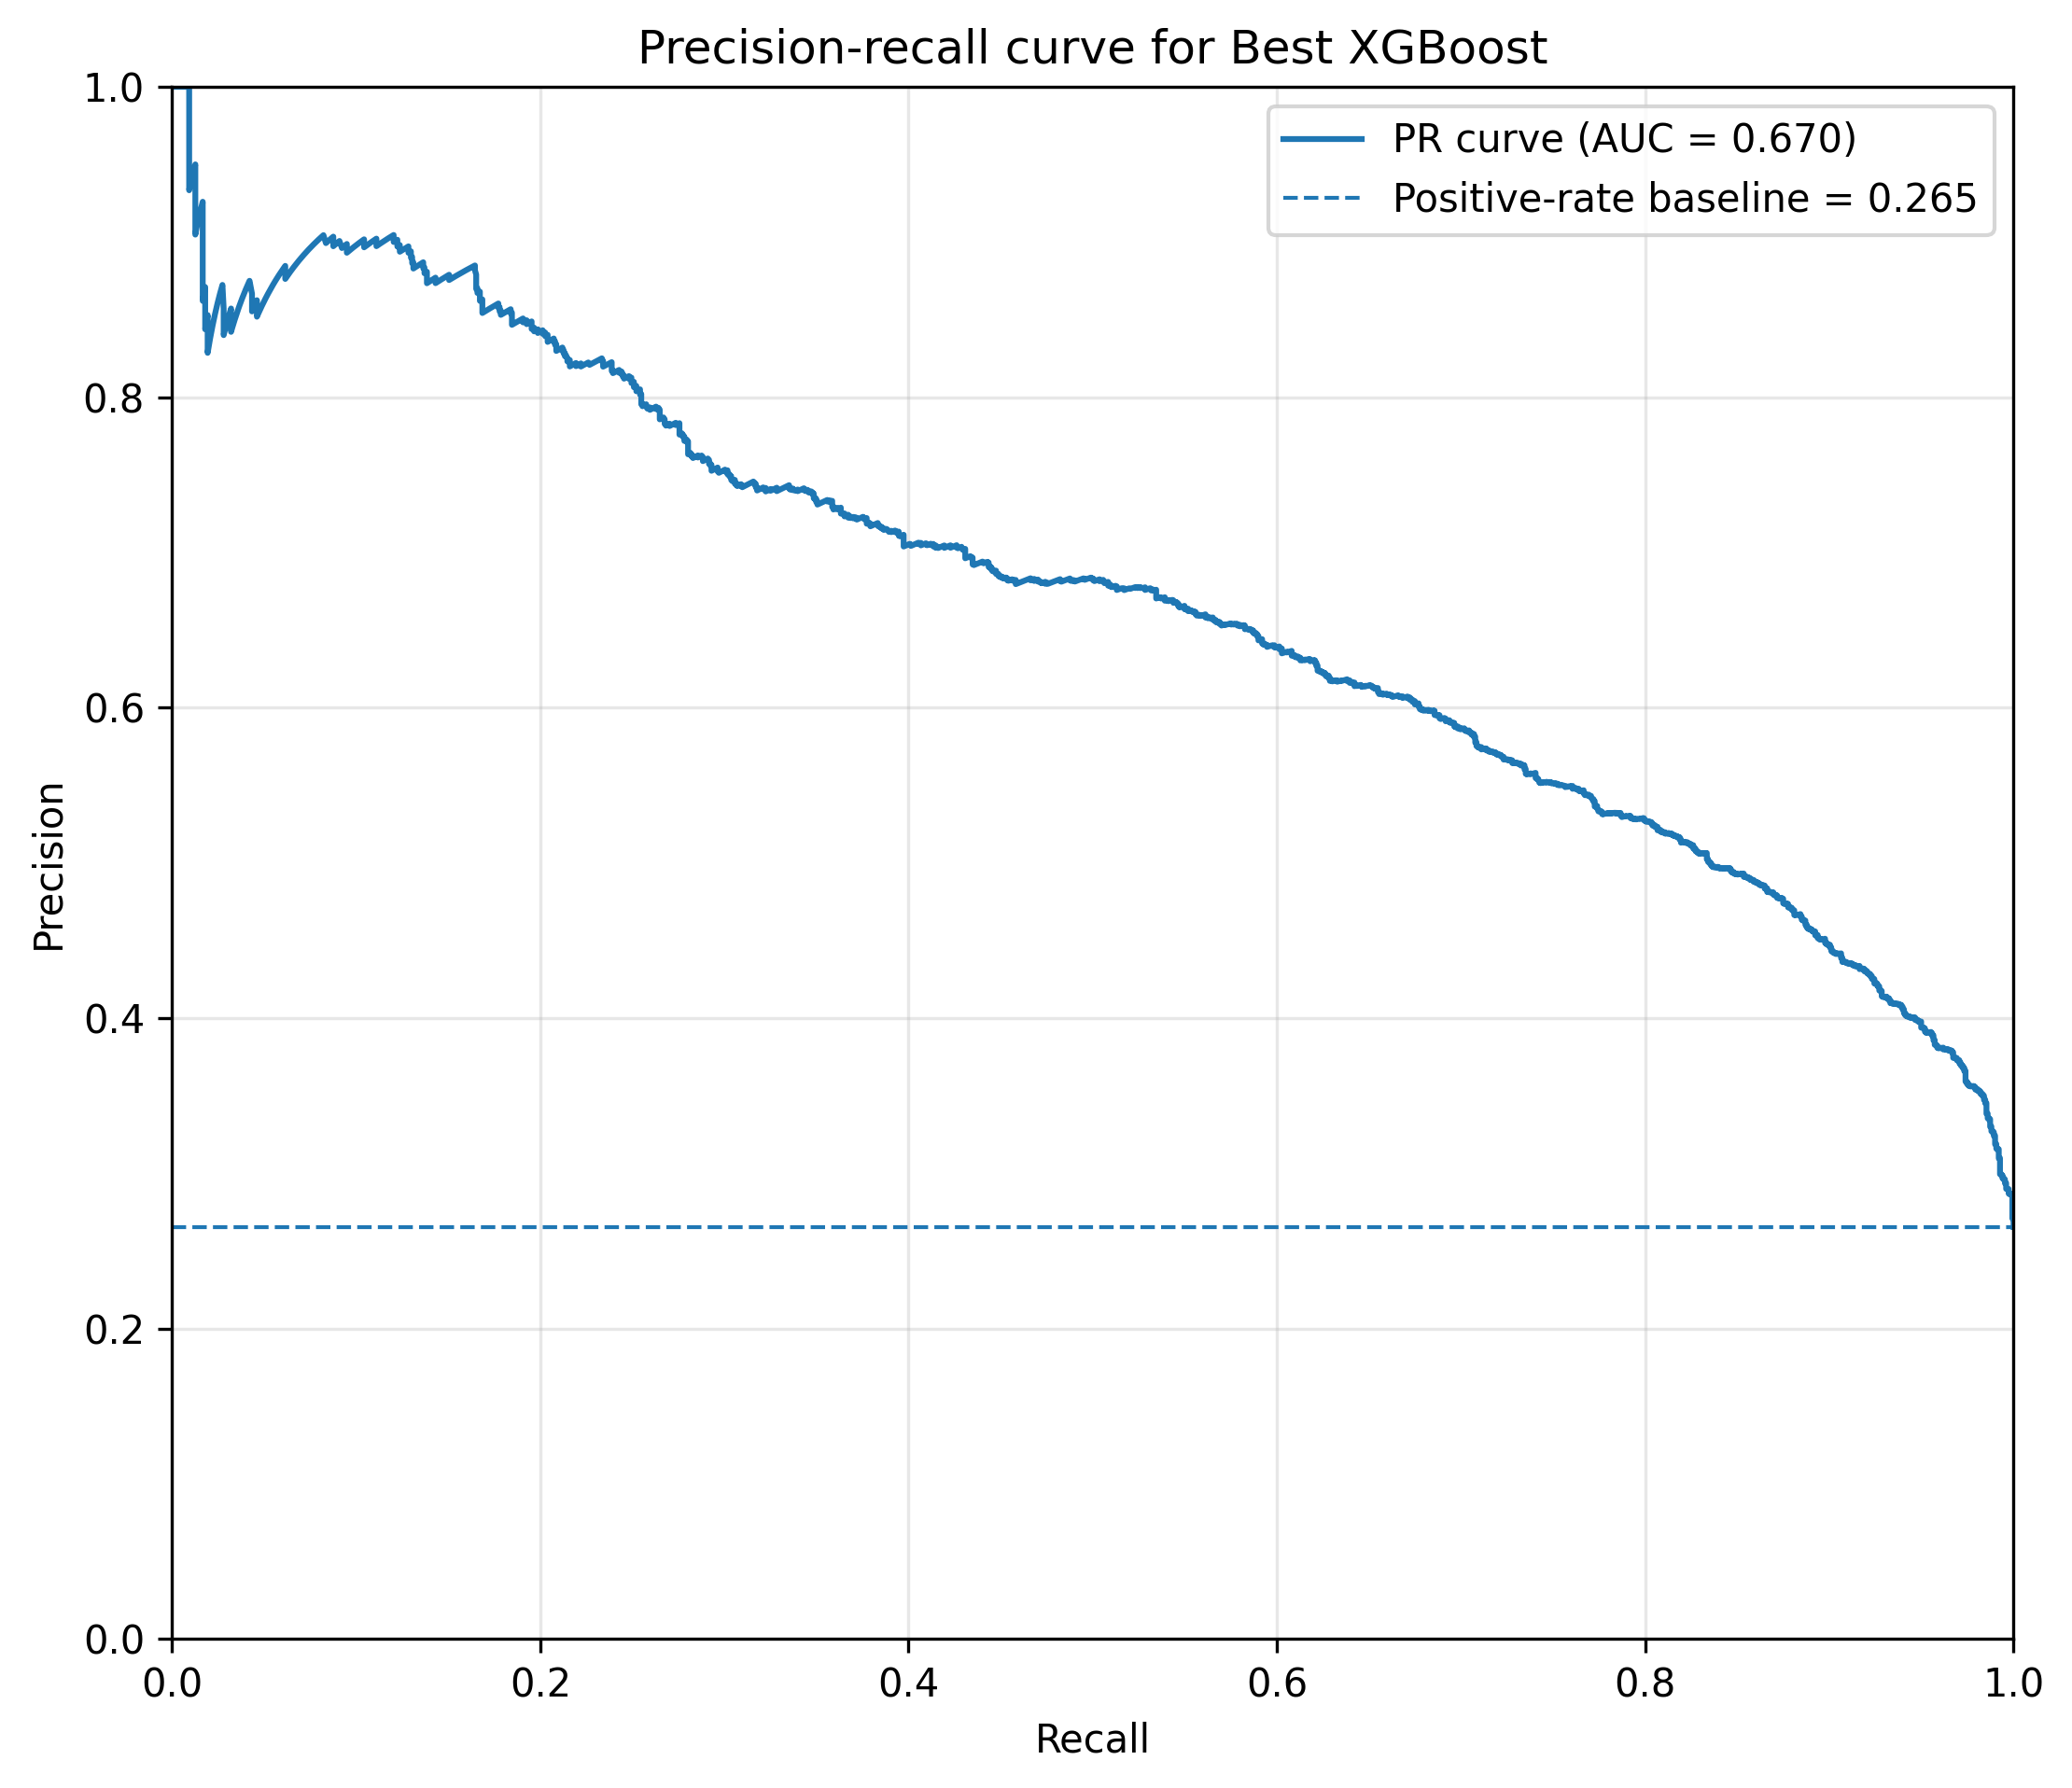
\includegraphics[width=0.82\textwidth]{../figures/boosting_precision_recall_curve.png}
\caption{Precision-recall curve for the selected XGBoost model}
\label{fig:boosting-pr-curve}
\end{figure}

The PR curve is especially relevant because churn is the positive minority class. The curve shows that precision is high for the top-ranked customers, then declines as recall approaches one. This is the normal shape of a useful risk-ranking model: the highest-score customers are enriched for churn, while extending intervention to lower-score customers gradually approaches the base churn rate.

\subsection{Feature importance}

Feature importance is computed by refitting selected boosting candidates on the full training set. This refit is used only for interpretation and does not enter the performance estimates. For the selected XGBoost model, the largest importance is assigned to the month-to-month contract indicator. Other important predictors include online security absence, fiber optic internet service, electronic-check payment, tech-support absence, long-term contract indicators, and tenure.

\begin{table}[H]
\centering
\small
\begin{tabular}{lr}
\toprule
Feature & Importance \\
\midrule
Contract\_Month-to-month & 0.418 \\
OnlineSecurity\_No & 0.104 \\
InternetService\_Fiber optic & 0.100 \\
PaymentMethod\_Electronic check & 0.071 \\
TechSupport\_No & 0.060 \\
Contract\_Two year & 0.036 \\
tenure & 0.028 \\
StreamingTV\_Yes & 0.021 \\
PaperlessBilling\_No & 0.019 \\
Contract\_One year & 0.016 \\
\bottomrule
\end{tabular}
\caption{Top feature importances for the selected XGBoost model}
\label{tab:boosting-feature-importance}
\end{table}

\begin{figure}[H]
\centering
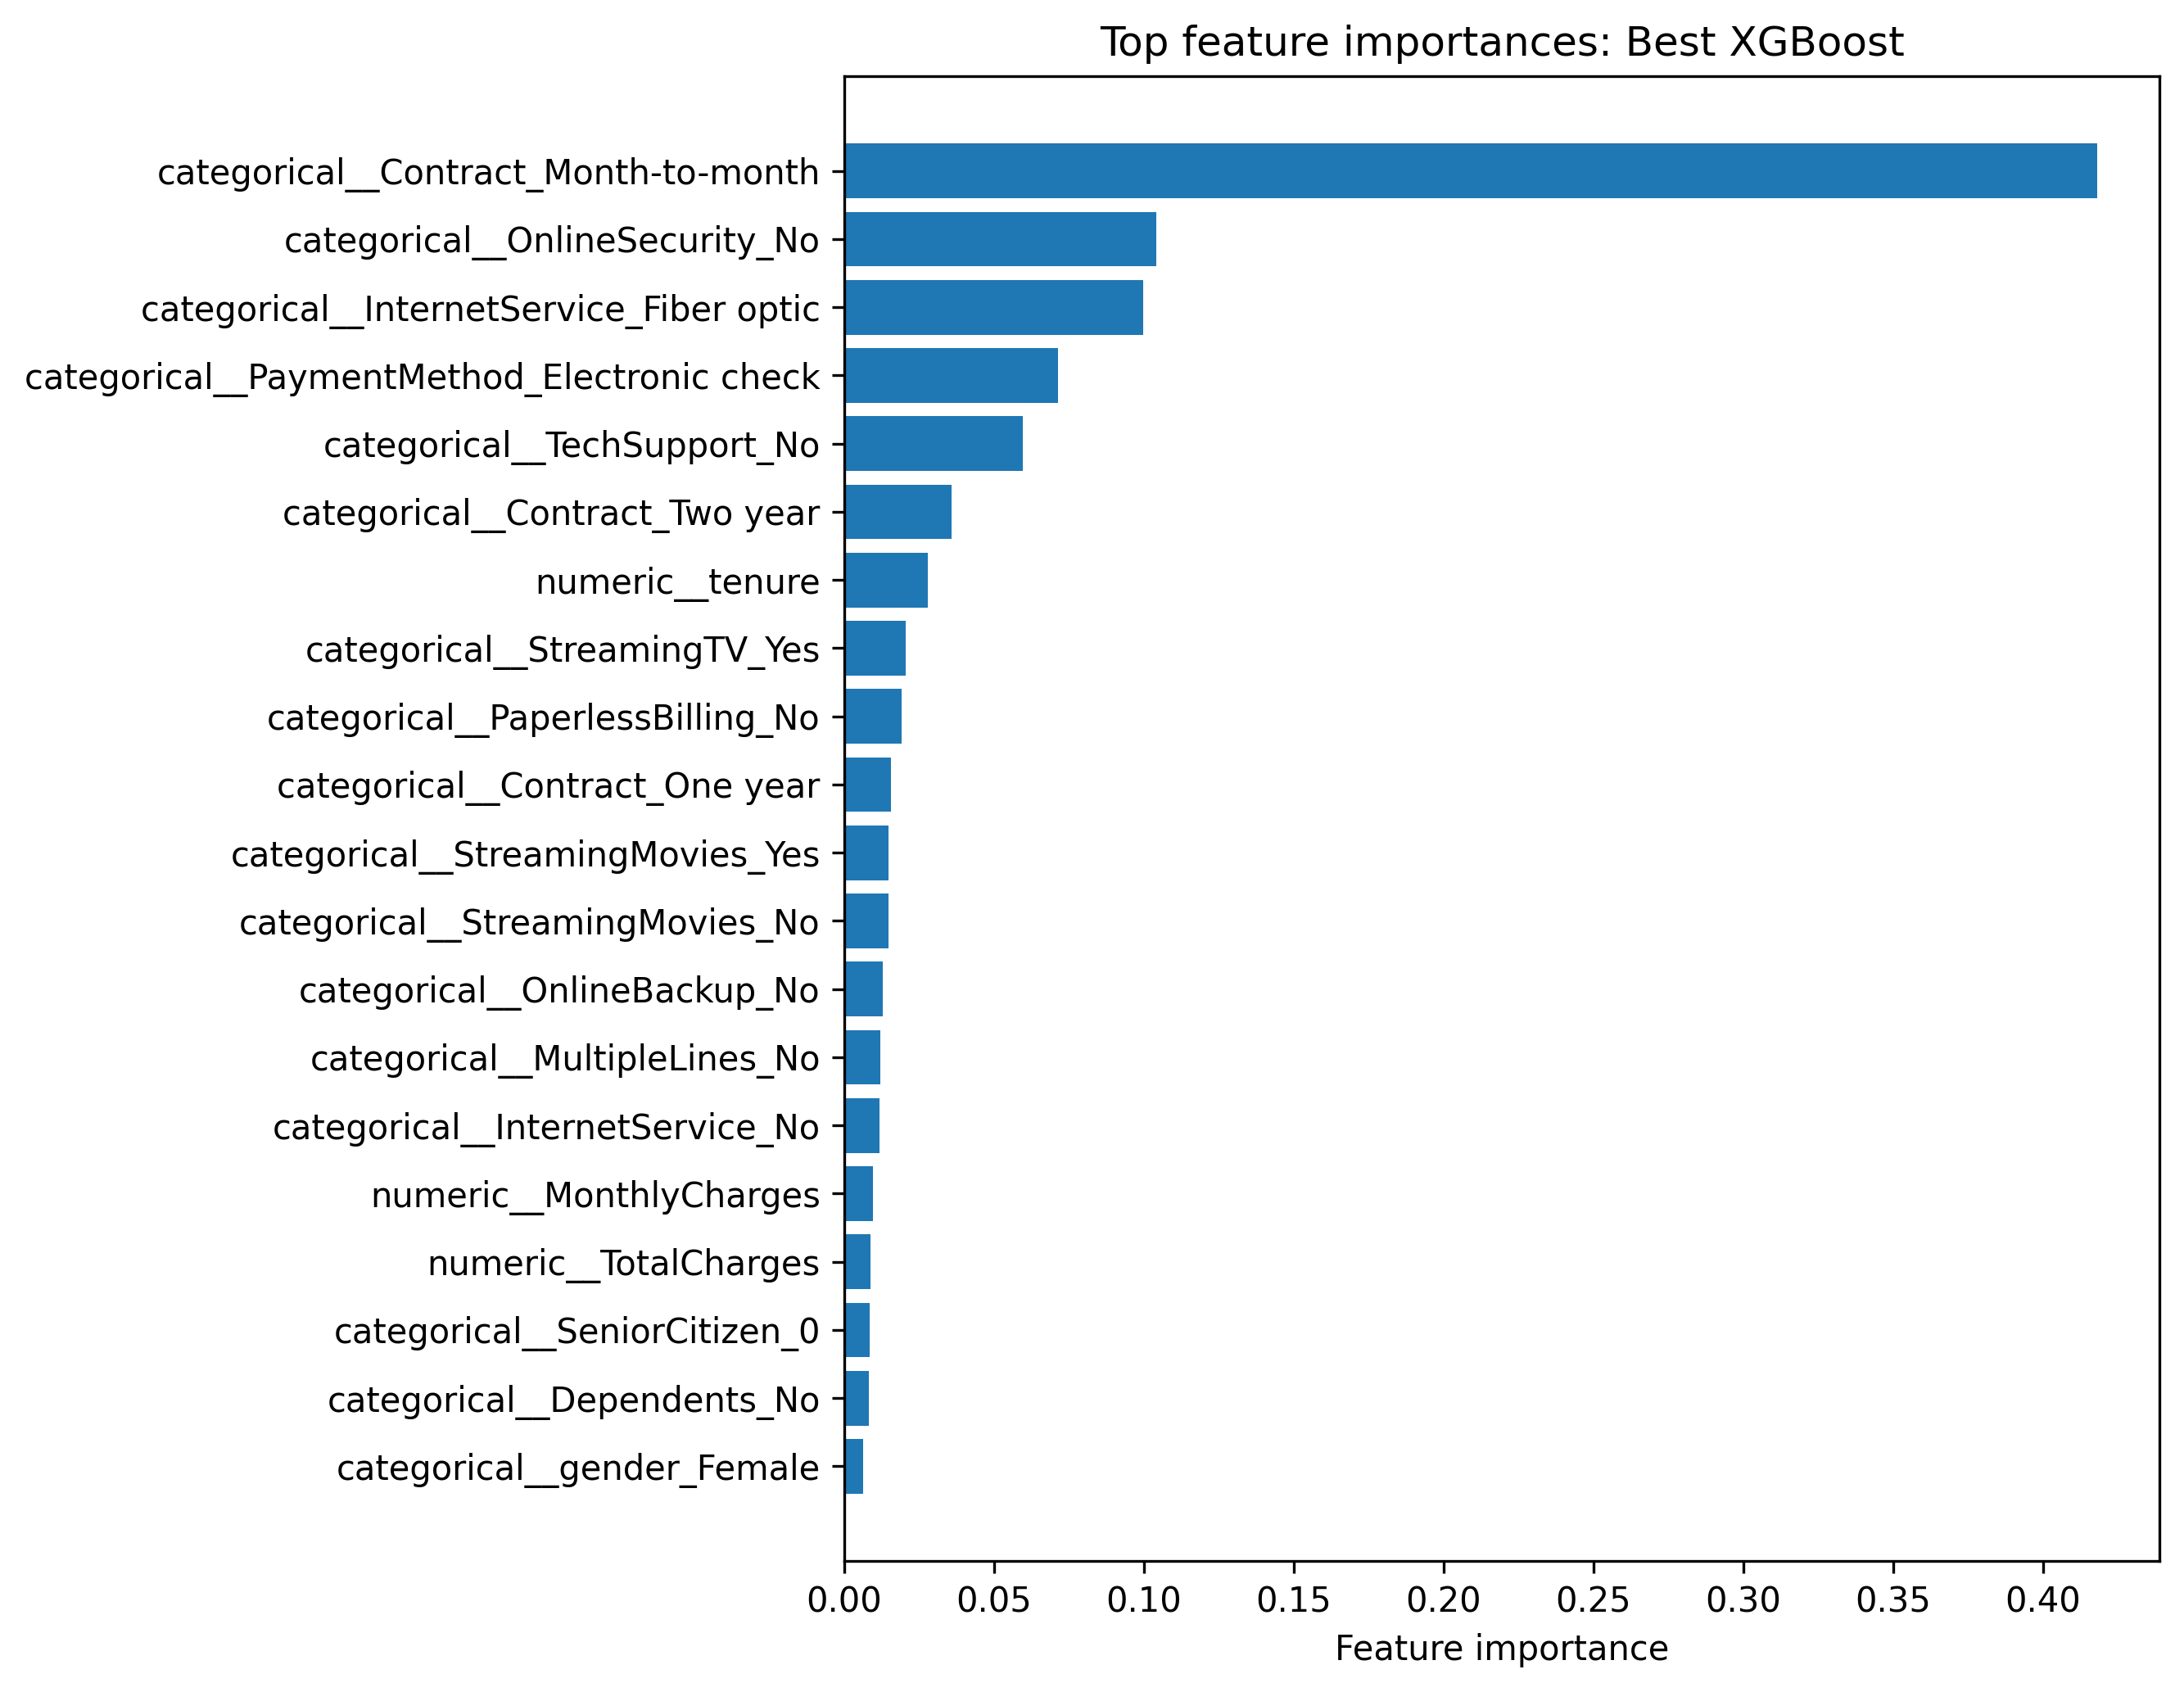
\includegraphics[width=0.84\textwidth]{../figures/boosting_feature_importance.png}
\caption{Top feature importances for the selected XGBoost model}
\label{fig:boosting-feature-importance}
\end{figure}

These importances are consistent with earlier sections. Contract type, tenure, internet service, online security, tech support, and payment method have repeatedly appeared as strong churn-related predictors. The feature importance values should not be interpreted causally. They describe how this fitted boosted-tree model uses features for prediction, not what would happen if a customer changed contract type or payment method.

\subsection{Section summary}

Boosting extends the tree-based modelling sequence by moving from independent averaging to sequential additive correction. The evaluated models include classical AdaBoost, scikit-learn gradient boosting, histogram gradient boosting, XGBoost, LightGBM, and CatBoost.

The development-stage results show that boosting is a strong model family for this tabular churn problem. The selected XGBoost candidate has the highest pooled out-of-fold PR-AUC, approximately \(0.670\), followed very closely by \texttt{GradientBoostingClassifier} and CatBoost. The fixed-grid selection table gives CatBoost the highest mean CV PR-AUC, but the difference relative to XGBoost and GradientBoosting is extremely small. The safe conclusion is therefore that boosted tree methods form a strong group, not that one specific implementation has been proven best.

Compared with earlier references, boosting clearly improves over the single decision tree and modestly improves over the selected bagged trees, selected random forest, and selected L2 logistic regression. The improvement is meaningful enough to keep boosted trees as serious final candidates, but not large enough to ignore uncertainty, tuning fairness, threshold selection, or calibration. Those issues remain part of the later final model-comparison stage, which will compare the strongest model families under a more deliberate training-only selection procedure before the held-out test set is used.
